\documentclass{article}

\usepackage[utf8]{inputenc}
\usepackage{graphicx}
\usepackage{geometry}   \geometry{margin=1in}
\usepackage{amsmath}
\usepackage{xcolor}
\usepackage{float}
\usepackage{longtable}
\usepackage{multirow}
\usepackage{natbib}
\usepackage[nonumberlist]{glossaries}
\makeglossaries
\loadglsentries{glossary}


\title{Hot Swappable Pedalboard and Routing System:\\Progress Report 4}
\author{Nicholas Pham}
\date{February 2019}

\begin{document}

\maketitle
\begin{center}
    Electrical Engineering \\
    Scott Kuindersma, Jim MacAurthur
\end{center}

\newpage
\glsaddall
\printglossaries
\newpage


\color{gray}
\section{Define}
	\subsection{Introduction}
	
	Many electric guitarists use effect pedals to augment their guitar amp's sound.  First developed in the 1960s, there are now thousands of pedals available for guitarists to use.  Because of the plethora of options, guitarists need an easy way to compare and interchange effects.

	In my project proposal, I proposed an integrated \emph{hot-swappable} guitar effect pedalboard and switching unit to improve the efficiency by which guitarists can change out their effects pedals to create new sounds.  The proposal focused on two main use cases: performing musicians who need to quickly change sounds, and studio musicians who need ways to radically alter their sound via new combinations of effects.

	Through discussions with my advisors, the focus of this project has shifted away from the first use model to an expanded version of the second.  Following the first step of the design process \cite{ES100Lec3}, marketing, led to this shift of focus, as there are already products available that allow performing musicians to program combinations of effects to be switched on and off at once.  Now the product will aim less to be portable and usable in real-time by a gigging musician and more useful for off-line effects swapping.  As will be further described in the next section, the product will be designed as a sales tool for retailers such as Guitar Center who sell guitar effects pedals.  By making it easier for customers to try out new combinations of pedals, this product will help retailers sell more units, and help customers discover and purchase additional processors to expand and improve their guitar systems.
	

	\subsection{Motivation and Use Cases}

	
	Though in an age of Internet shopping there are many guitar related products available for purchase on-line, most players want to test potential purchases in person before buying them.  As such, brick-and-mortar music stores such as Guitar Center still have a place in the industry.
	\subsection{Testing Effects}
	The existing method for testing effects pedals at brick-and-mortar retail store such as Guitar Center is a slow process.  Once a customer requests to test a pedal, an employee brings the particular unit being test to a padded table (see Figure \ref{fig:GuitarCenterBoard}.  The employee must also find the correct power supply before connecting the unit to the guitar and the amplifier.  If a customer would like to test two pedals, for instance to decide between them which one to purchase, the employee would need to grab an additional power supply and cable for connection.  Then to perform an A-B test, the customer must turn the amplifier output off to prevent pops before disconnecting the current pedal and replacing it with the other one.  This time required for swapping the pedals limits the customer's ability to accurately judge the relative qualities of the units under test.  This cost can result in several negative consequences.  First, because of the reduction in accuracy of the A-B test, the guitarist may not be able to make a well-informed decision as to which effect best suits them, which could result in them either purchasing an inferior product, or in them deciding not to purchase any product at all.  Second, the known difficulties of testing effects pedals in this way may deter potential customers from even bothering at all, which limits the number of "impulse" purchases.  An improved method for testing guitar effects pedals at guitar stores would be beneficial to both consumers of these effects and their producers and retailers.

	\begin{figure}
		\centering
		\includegraphics[width = 0.4\textwidth]{PR2Images/GuitarCenterBoard.jpg}
		\caption{A typical "test bench" for most guitar pedals.  Guitar Center, Boston MA, September 2018.}
		\label{fig:GuitarCenterBoard}
	\end{figure}

	\subsection{Sales Displays}
	While most of the in-stock effects pedals at retailers like Guitar Center are stored in a display for customers to peruse, some larger companies have integrated displays of their products.  For example, Figure \ref{fig:BossDisplay} shows one such display, containing products from Boss, one of the most popular companies in the industry \cite{ReverbMostPopular}.  As can be seen, the pedals are permanently attached to the display board, and are connected in series with power available to all effects at once.  This solves some of the issues mentioned previously.  For pedals that are available in these displays, employees do not need to do anything for customers to test them.  Customers must only plug a guitar into an input to the display unit, which automatically connects to the first pedal.  The last pedal in the series chain is always connected to a guitar amp.

	\begin{figure}
		\centering
		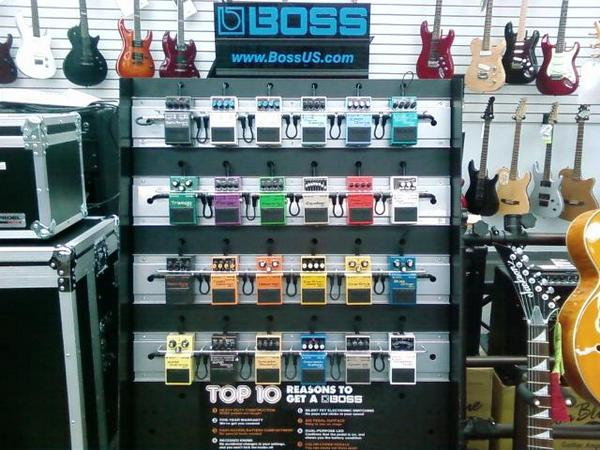
\includegraphics[width = 0.6 \textwidth]{PR2Images/BossDisplay.jpg}
		\caption{A display of Boss pedals typical to those found at retail stores such as Guitar Center \cite{BossDisplayPhoto}}
		\label{fig:BossDisplay}
	\end{figure}

	However, this system does have some limitations.  The first issue stems from the bypass method of many of these units.  Many guitar pedals, including all products offered by Boss, include a buffer that is active when the main "effect" is bypassed (see Figure \ref{fig:BufferedBypassConfig}).  This is useful for performing guitarists who often use cables totaling up to fifty feet in length.  The capacitive loading from the coaxial cable can result in high frequency loss, as guitar pickups can have DC output resistance on the order of $10k\Omega$.  A high input impedance and low output impedance buffer placed closer to the guitar can reduce the effects of this high frequency roll-off, which is typically undesirable.  However, because these display boards can contain up to thirty or more effects, there can be issues with signal degradation \cite{OrmanBypassMeasurements}.  This results in an inaccurate representation of the sound of any single pedal in the display.

	\begin{figure}
		\centering
		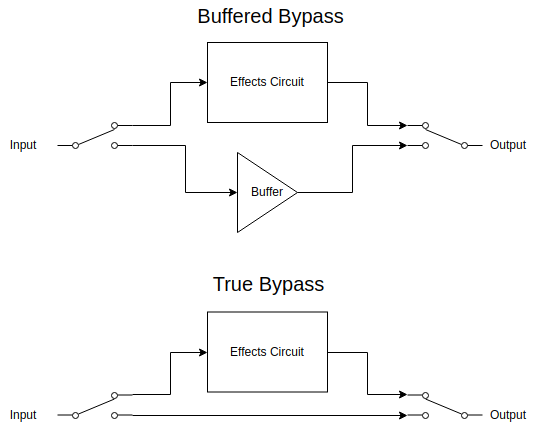
\includegraphics[width = 0.6 \textwidth]{PR2Images/BufferedvTrueBypass}
		\caption{Comparison of Buffered Bypass vs True Bypass topologies.  With the former, a buffer is in still placed in the signal even when the effect circuit is bypassed (some forms include the buffer prior to the effects circuit so the input is always buffered).  The true bypass topologies mechanically bypasses the effect circuit with a wire.}
		\label{fig:BufferedBypassConfig}
	\end{figure}


	Another issue is the fixed order and routing of the effects in the display.  The connection topologies between effects units can result in radical differences in output, which can affect the perceived quality of a pedals sound, when used in conjunction with others.  For example, consider the different topologies for connecting a distortion and delay pedal in Figure \ref{fig:PedalConnectionTopologies}.  The first one shows the guitar connected to the distortion pedal, which has its output connected to the input of a delay pedal, which in turn is connected to the guitar amplifier.  In this case, the sound might be the main distorted guitar sound with some dying echoes of the distorted sound.  The second topology shows the guitar connected to the distortion and delay pedals in parallel, which would result in the main distorted guitar sound and echoes of the "clean", unaffected guitar.  Finally, the third case shows the guitar first connected to the delay, which is them connected in series with the distortion pedal.  In this case, though the repeats of the delay decrease in amplitude over time, the non-linear clipping of the distortion pedal results in the echoes sounding at equal volume, all heavily distorted.  As can be seen even with this simple example involving only two effects, there are a multitude of possible connection topologies typically available to guitarists who own guitar pedals that are not available for testing on such display boards.

	\begin{figure}
		\centering
		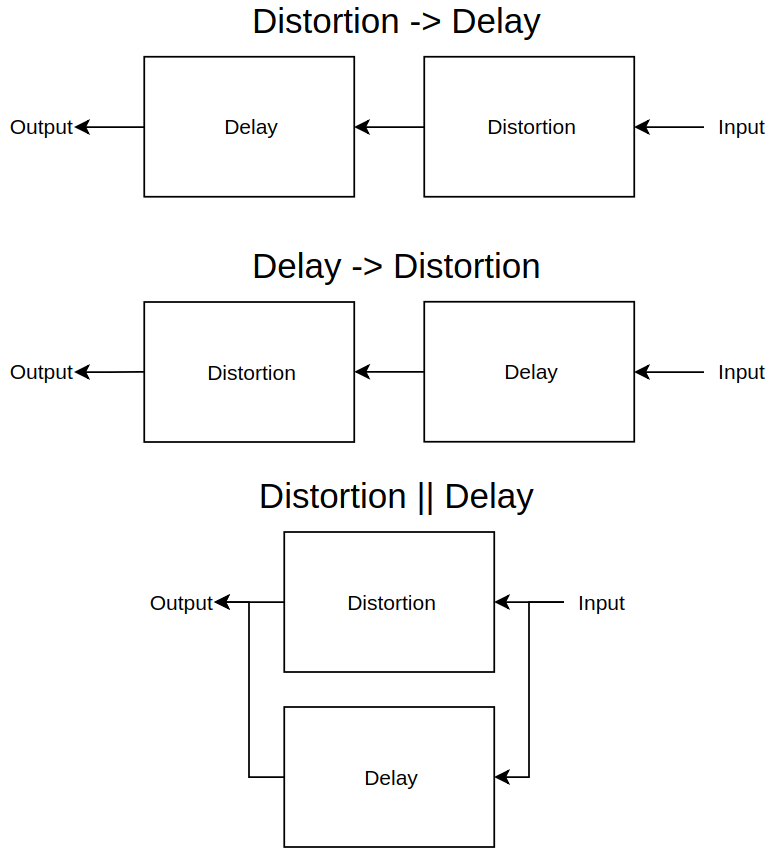
\includegraphics[width = 0.4 \textwidth]{PR2Images/RoutingConfigs.png}
		\caption{Example of the different ways to combine just two pedals.  More than two effects will have exponentially more options}
		\label{fig:PedalConnectionTopologies}
	\end{figure}

	\subsection{Studio Musicians}

	While this discussion has so far focused on guitarists as customers in a store, the same issues can face studio musicians hired for recordings.  These musicians must be able to produce any tone that their boss, the producer or artist who hired them, wants for the recording.  Because studio and musician time is very expensive, these studio musicians may have limited time to decide on and set up their equipment before recording begins.  Typically they might plug in pedals individually much as a customer does at a guitar store, which shares the issues described above.  Alternatively, some studio musicians might have their effects pedals integrated into an automatic switching system alluded to in the Overview.  However, these systems are often not intuitive to program, which means that the musician may set up a limited number of "presets", combinations of effects, that they will use.  This can limit their creativity in developing new sounds for their recordings.  A more intuitive system for connecting the effects pedals they already own would facilitate their creativity and save money by reducing the time spent on the mechanics of changing out equipment.
	

	\subsection{Prior Art}
	

	In addition to the displays mentioned above, there are several patents related to this project.

		\subsubsection{Magnetic Pedal Attachment}
		The Earthboard from Rare Earth Music LLC uses a unique system of magnets both to attach pedals to the pedalboard and to provide simple power to them.  Pedals are attached on a plate via a hook and loop device such as velcro.  Then the plates magnetically attach to long metal rails.  The two rails provide 9VDC power to the pedals via cabled connections between pedal and plate \cite{EARTHBOARDSITE}.

		\subsubsection{Bracket Attachment}

		U.S. Patent Grant US9620094B2 describes an improved method for attaching pedals to a pedalboard \cite{ABBATE:2016}.  Using small brackets which are directly mounted to the pedal enclosure via the bottom cover screws, this method for mounting pedals is much more stable and solid than velcro or zip-tie methods, while also using few external materials. However, this implementation describes directly attaching the pedals to the pedalboard, which will require other screws. This means the pedal placement will be fairly permanent and it will be difficult to swap out pedals, necessitating the use of external tools such as a screwdriver.

		\subsubsection{Modular Effect System}

		U.S. Patent US4479238A describes an effect system incorporating a main parent enclosure which contains power and signal routing circuits and receiving slots for effect modules \cite{SPECTOR:1982}. These modules contain effects circuits built into a special form factor that allows them to be inserted into the slots and make signal and power connections with the main unit. The main enclosure contains routing circuits which can choose, remotely or on the front panel, which effects should be connected, much like the automatic routing systems described previously. In addition, the housing automatically bypasses any slot in which no module is fully inserted, preventing issues with ”hot-swapping”, or removing the effect card while the system is in use. This system does a nice job of allowing different combinations of effects to be tested, but it does have a significant limitation. The effect modules must be of the correct card format, which limits the user to specifically designed units. As the guitar pedal form factor is so ubiquitous (though not exactly standardized: pedals may come in many shapes and sizes), a guitarist using this system would not be able to incorporate the majority of effects units offered today, and would not be able to use any pedals they already own. In addition, because of their design, these card modules cannot be used in absence of the main enclosure unlike normal guitar pedals, further limiting their flexibility.

		\subsubsection{Waterproof Swappable Effects System}

		U.S. Patent USD782567S1 describes a pedalboard system which allows guitar effects pedals to be attached magnetically to a pedalboard \cite{FAORO:2015board}.  The system allows for hot-swappability of effects, which are connected to the board's internal routing via contacts underneath: no external cables are required.  While the patent has very little detail on the capabilities and specifications of the product, it is available for sale from Nexi Industries \cite{NexiIndustries}.  Their website claims that the switching in both the pedals and on the board is "true bypass", which in industry terminology means that the effects circuits are mechanically switched out of the signal path when bypassed, as opposed to electronic switching with buffers mentioned above.  The initial system was designed to be used specifically with proprietary effects pedals, covered in U.S. Patent USD782566S1 \cite{FAORO:2015pedal}.  However, the manufacturer has since released a product to interface with third-party guitar effects \cite{conNEXI}.

		The product does offer a solution to many issues thus far described.  In particular, it allows for fast swapping of effects pedals without the need for unplugging signal and power cables.  However, it does have some issues.  The interface between the pedal and the plate still relies on uncontrolled lengths of cable required to make connections with the pedal's input and output jacks.  The system also supposes a single power supply type, 9VDC through a 2.1 mm center negative plug.  While this is fairly standard, there are a number of popular effects, particularly more powerful digital ones, that require different power supplies.  There is also no improvement on the mechanism for attaching third party effects to the plates: the marketing examples show zip-ties being used, which can damage the pedal \cite{conNEXI}.  The pedal plates also only come in one size which is not suitable for many larger pedals.  Finally, the system supports only a single series routing option, which eliminates many possible routing topologies.

	

	\subsection{Specifications}
	The main issue with the current system of testing guitar pedals is the inconvenience and speed of switching between different units.  The following specifications directly relate to reducing the inconvenience and time required to swap between different units when demoing.

	\begin{center}
	\renewcommand{\arraystretch}{1.5}
	\begin{tabular}{|l|l|l|p{6cm}|}
		\hline
		Metric & Min Target Value & Preferred Target & Justification \\
		\hline
		Swapping Time & 80\% reduction & 90\% & To be useful, the solution should offer a major improvement in swap time.  As current swap time is on the order of 10 seconds, the improved switching time should be on the order of 1 second.\\
		Compatibility &  $>$80\% & $>$ 95\% & In order to be an effective tool, the solution must be usable with a majority of pedals available at typical retail locations.  80\% is reasonable because a majority of retailer stock contains pedals by a handful of brands.  There is a trade-off between compatibility versus function and form, so designing for any possible pedal is not possible. \\
		Intuition & $< 250$ words& $< 150$ words & In order to quantify the ease of use and intuitiveness of using the solution, a simple metric might be number of words required to give working knowledge in a user guide.  If the solution is easy to use and intuitive, it should not take long to teach a new user how to operate it.  250 words can easily fit on a double-spaced page, and most people can speak about 150 words per minute. \\
		\hline
	\end{tabular}
	\end{center}

	After these primary specification follow several additional requirements which ensure that the solution will be useful.

	\begin{center}
	\renewcommand{\arraystretch}{1.5}
	\begin{longtable}{|l|l|l|p{6cm}|}
		\hline
		Metric & Min Target Value & Preferred Target & Justification \\
		\hline
		System Cost & \$200 & \$100 & Though the price of the solution when sold to a retailer is dependent on marketing and other factors, the cost to produce the system should be relatively low, so as to make it a viable option for use as a sales tool. \\
		Incremental Cost & \$20 & \$1 & There must also be a distinction drawn between the cost of an entire system and the cost of allowing an additional pedal to interface with the system.  Because many retail stores may stock hundreds of guitar pedals, the cost of adding a single new pedal to the system must be a small percent of that pedal's cost. \\
		Signal-to-Noise Ratio & 90dB &  120dB & The electric guitar, by virtue of its simple passive magnetic pickups can have a very high SNR, measured in non-ideal circumstances at +90 dBV.  Higher values in a controlled environment are likely.  Though many guitar pedals may have lower SNRs, it is vital the solution maintain the maximum possible dynamic range. \\
		Frequency Response & 20 - 20 kHz & DC - 30 kHz & As an audio system, the solution must at minimum pass the audio range.  Because the solution might be used with processors that could output DC voltages (such as control voltage signals), the frequency response should extend down to DC.  Ideally, the frequency response would exceed 20kHz to allow for higher frequency components generated by the guitar and nonlinear effects pedals. \\
		Switching Time & 125 ms & 20 ms & When swapping a pedal in or out of the system, there should be no perceptible delay between when the pedal is inserted and when the sound becomes effected.  125 ms is the threshold for detectability of sound latency against visuals \cite{Timing}.  An ideal target would be in the range of tens of milliseconds, below which the Precedence effect suggests that there would be little discontinuity heard \cite{PrecedenceEffect}. \\
		Transient & $<$0.5 dB & $<$ 0.1 dB & When swapping a pedal in or out of the system, any transient created must not damage connected equipment (such as the amplifier) or be disturbing. \\
		SELV compliance	& Yes & - & For ease of design and safety, the solution should accept DC voltage from an external AC/DC converter.  Through Separated Extra Low Voltage (SELV) compliance, the solution will not need to design for high voltage safety, which would reduce design and regulation/testing costs. \\
		\hline
	\end{longtable}
	\end{center}

\section{Design}
	\subsection{System Level Description}

	Though it may appear trivial at first, the broad scope of the design space of this project means making difficult design decisions where there is often no clear answer.  One of the biggest up front challenges is in developing the method to standardize the physical and electrical connections that will be used for the hot swapping feature.  

	Data collected during a site visit to a Guitar Center retail location in Boston demonstrated the plethora of effects pedals available at brick-and-mortar stores \cite{MyPedalData}.  These 150 guitar pedals represent a good mix of products, from mass market production units such as the Boss DS-1 to high quality and expensive effects like Eventide's H9.  While the major manufacturers like Boss, MXR, and Electro Harmonix have narrowed their form factors down to a handful of types each, there is no standardization across producers on features important for this project, including the dimensions of the enclosure, the location and orientation of the signal and power jacks, the location of the screws used to hold the pedal's bottom plates.  Though most products use the de facto standard 9 VDC, center negative power supply connected with a 2.1 mm plug, this too has variations in some cases \cite{MyPedalData}.  All of these variations complicate standardizing a form that can easily be hot swapped.

	\begin{figure}
		\centering
		\includegraphics[width = 0.6\textwidth]{PR2Images/GCpedals.jpg}
		\caption{Just some of the many pedals available on hand at Guitar Center, Boston MA.}
		\label{fig:GCpedalscase}
	\end{figure}

	The design process has focused on ease of use and intuition for the user over any other considerations where possible, which explains the preference for this tactile and tangible hot swapping method over some programmable switcher, as seen in \cite{ProgrammableSwitcherExample}.  This push for simplicity led to some increases in design complexity, including the need to automatically detect the hot swapping event rather than a separate user controlled switch.  The other major consideration was flexibility and a wide range of compatibility, though there were sometimes trade offs associated with supporting some less common features.

	To illustrate the main features and mechanisms of the solution, a block diagram is shown in Figure \ref{fig:SystemBlockDiagram}.  The individual blocks and their functions are summarized below.

	\begin{figure}
		\centering
		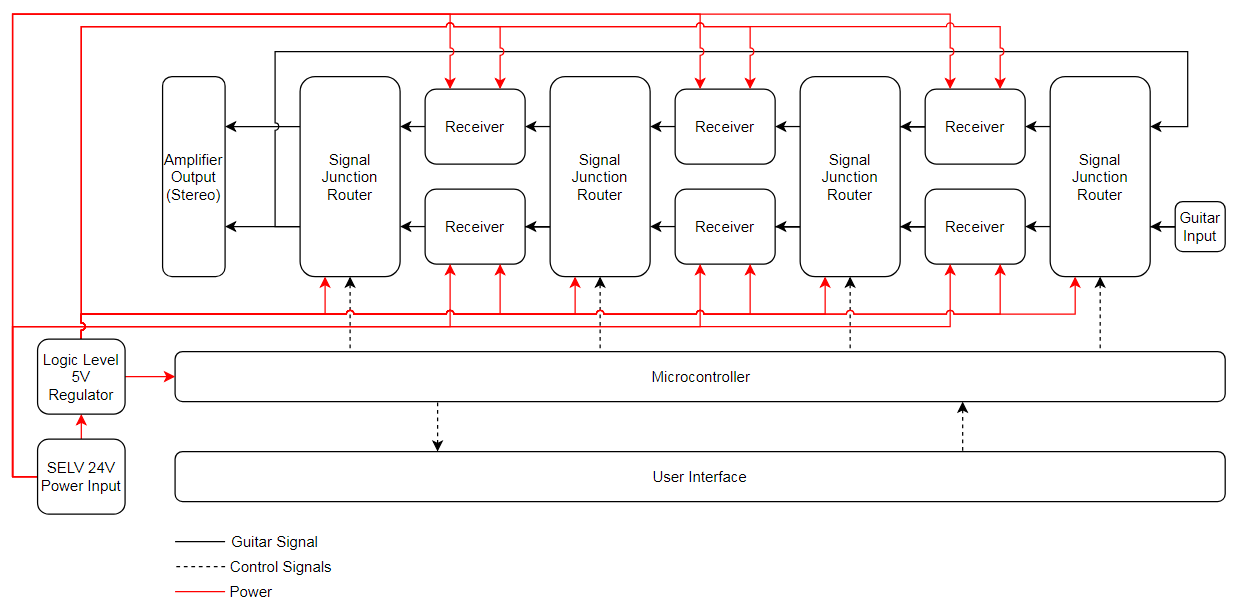
\includegraphics[width = \textwidth]{PR2Images/SystemBlockDiagram.PNG}
		\caption{Block Diagram of the Solution}
		\label{fig:SystemBlockDiagram}
	\end{figure}

	\subsubsection{Plate}
	Because of the large variety of guitar pedal shapes, they are not suitable for hot swapping in and out of a fixed receiving unit.  A simple and unobtrusive way to standardize their connections and physical form is through an interfacing plate.  To make ready for integration, a pedal will be outfitted with one of these trays on which it is mechanically attached.  The input, output, and power jacks are connected to the plate via short leads with standard plugs.  These leads can be removed and replaced to accommodate variations in plug location and size.  The plate makes these leads exposed to a standardized electrical interface for insertion into the hot swap receiver.

	\subsection{Receiver}
	A receiver is the dual of the plate.  It is a receptacle for a plate, and makes the necessary power and signal connections to allow the pedal to operate.  The receiver must also detect when a plate has been inserted or not.  When a plate is present, the receiver should send the guitar signal from its input to the plate, and return the output of the pedal coming from the plate to its output.  Otherwise, it should route the signal from its input straight to its output, bypassing the send/return loop.

	\subsection{Junction Signal Router}
	The signal routers are used to direct the outputs of certain receivers to the inputs of others to allow multiple pedals to be used at the same time.  The simplest router would be a single wire connecting the output of one receiver to the input of the next, but this limits the number of options available to make these signal connections.  The router should be as transparent to the signal as possible.

	\subsection{User Interface}
	The user can control a few functions of the product.  The primary one is the automatic bypassing of pedals when they are removed from plates.  The other major component is the communication of the current routing status and the ability of the user to control this routing.  These should strive to be as clear and intuitive as picking up the pedals.	
	
	\subsection{Design Choices}
		\subsubsection{Pedal-Plate Mounting}
		
			\paragraph{Through Screws}
			One important subsystem is the mounting of the pedals on their plates.  One attractive option is the use of screws through the pedal's bottom cover, as described in \cite{ABBATE:2016}.  This is the most visually simple technique, but relies on pedals that have similar screw hole locations.  As discussed below, while pedals from a single manufacturer tend to come in only a handful of form factors, the locations are not always standard across manufacturers.  In addition, some pedals do not have screws on opposite corners, which is required for a secure connection.  For instance, the Ibanez TS-9 Tubescreamer has bottom cover screws only on the upper (north) side of the pedal.  Because of this type of issue, the screw-through-plate method may not work for all pedals.  {
			In addition, to make use of the pedal's original screws, the plate material must be thin enough to allow the screws to pass through and still firmly grasp their threads.  This is discussed and accounted for in the choice of plate material.}

			\paragraph{Clamp}
			Another option for attaching pedals to their plates is via a clamping mechanism.  Figure \ref{fig:CornerClamp} shows a preliminary design for such a clamp, which would be used to attach pedals with irregular bottom screws.  The bracket would be located in x-y position by the bolt hole to the corner of the pedal, and would be firmly held down in the z direction by a bolt clamping through the plate. The inner sides of the bracket should be rubber or a similar surface that will not damage the finish of the pedal.  Because the screw method is compatible with so many effects, the clamp will not be pursued in the near future.  Only if a higher compatibility is required and time permits will this clamp method be examined further. 

			\begin{figure}
				\centering
				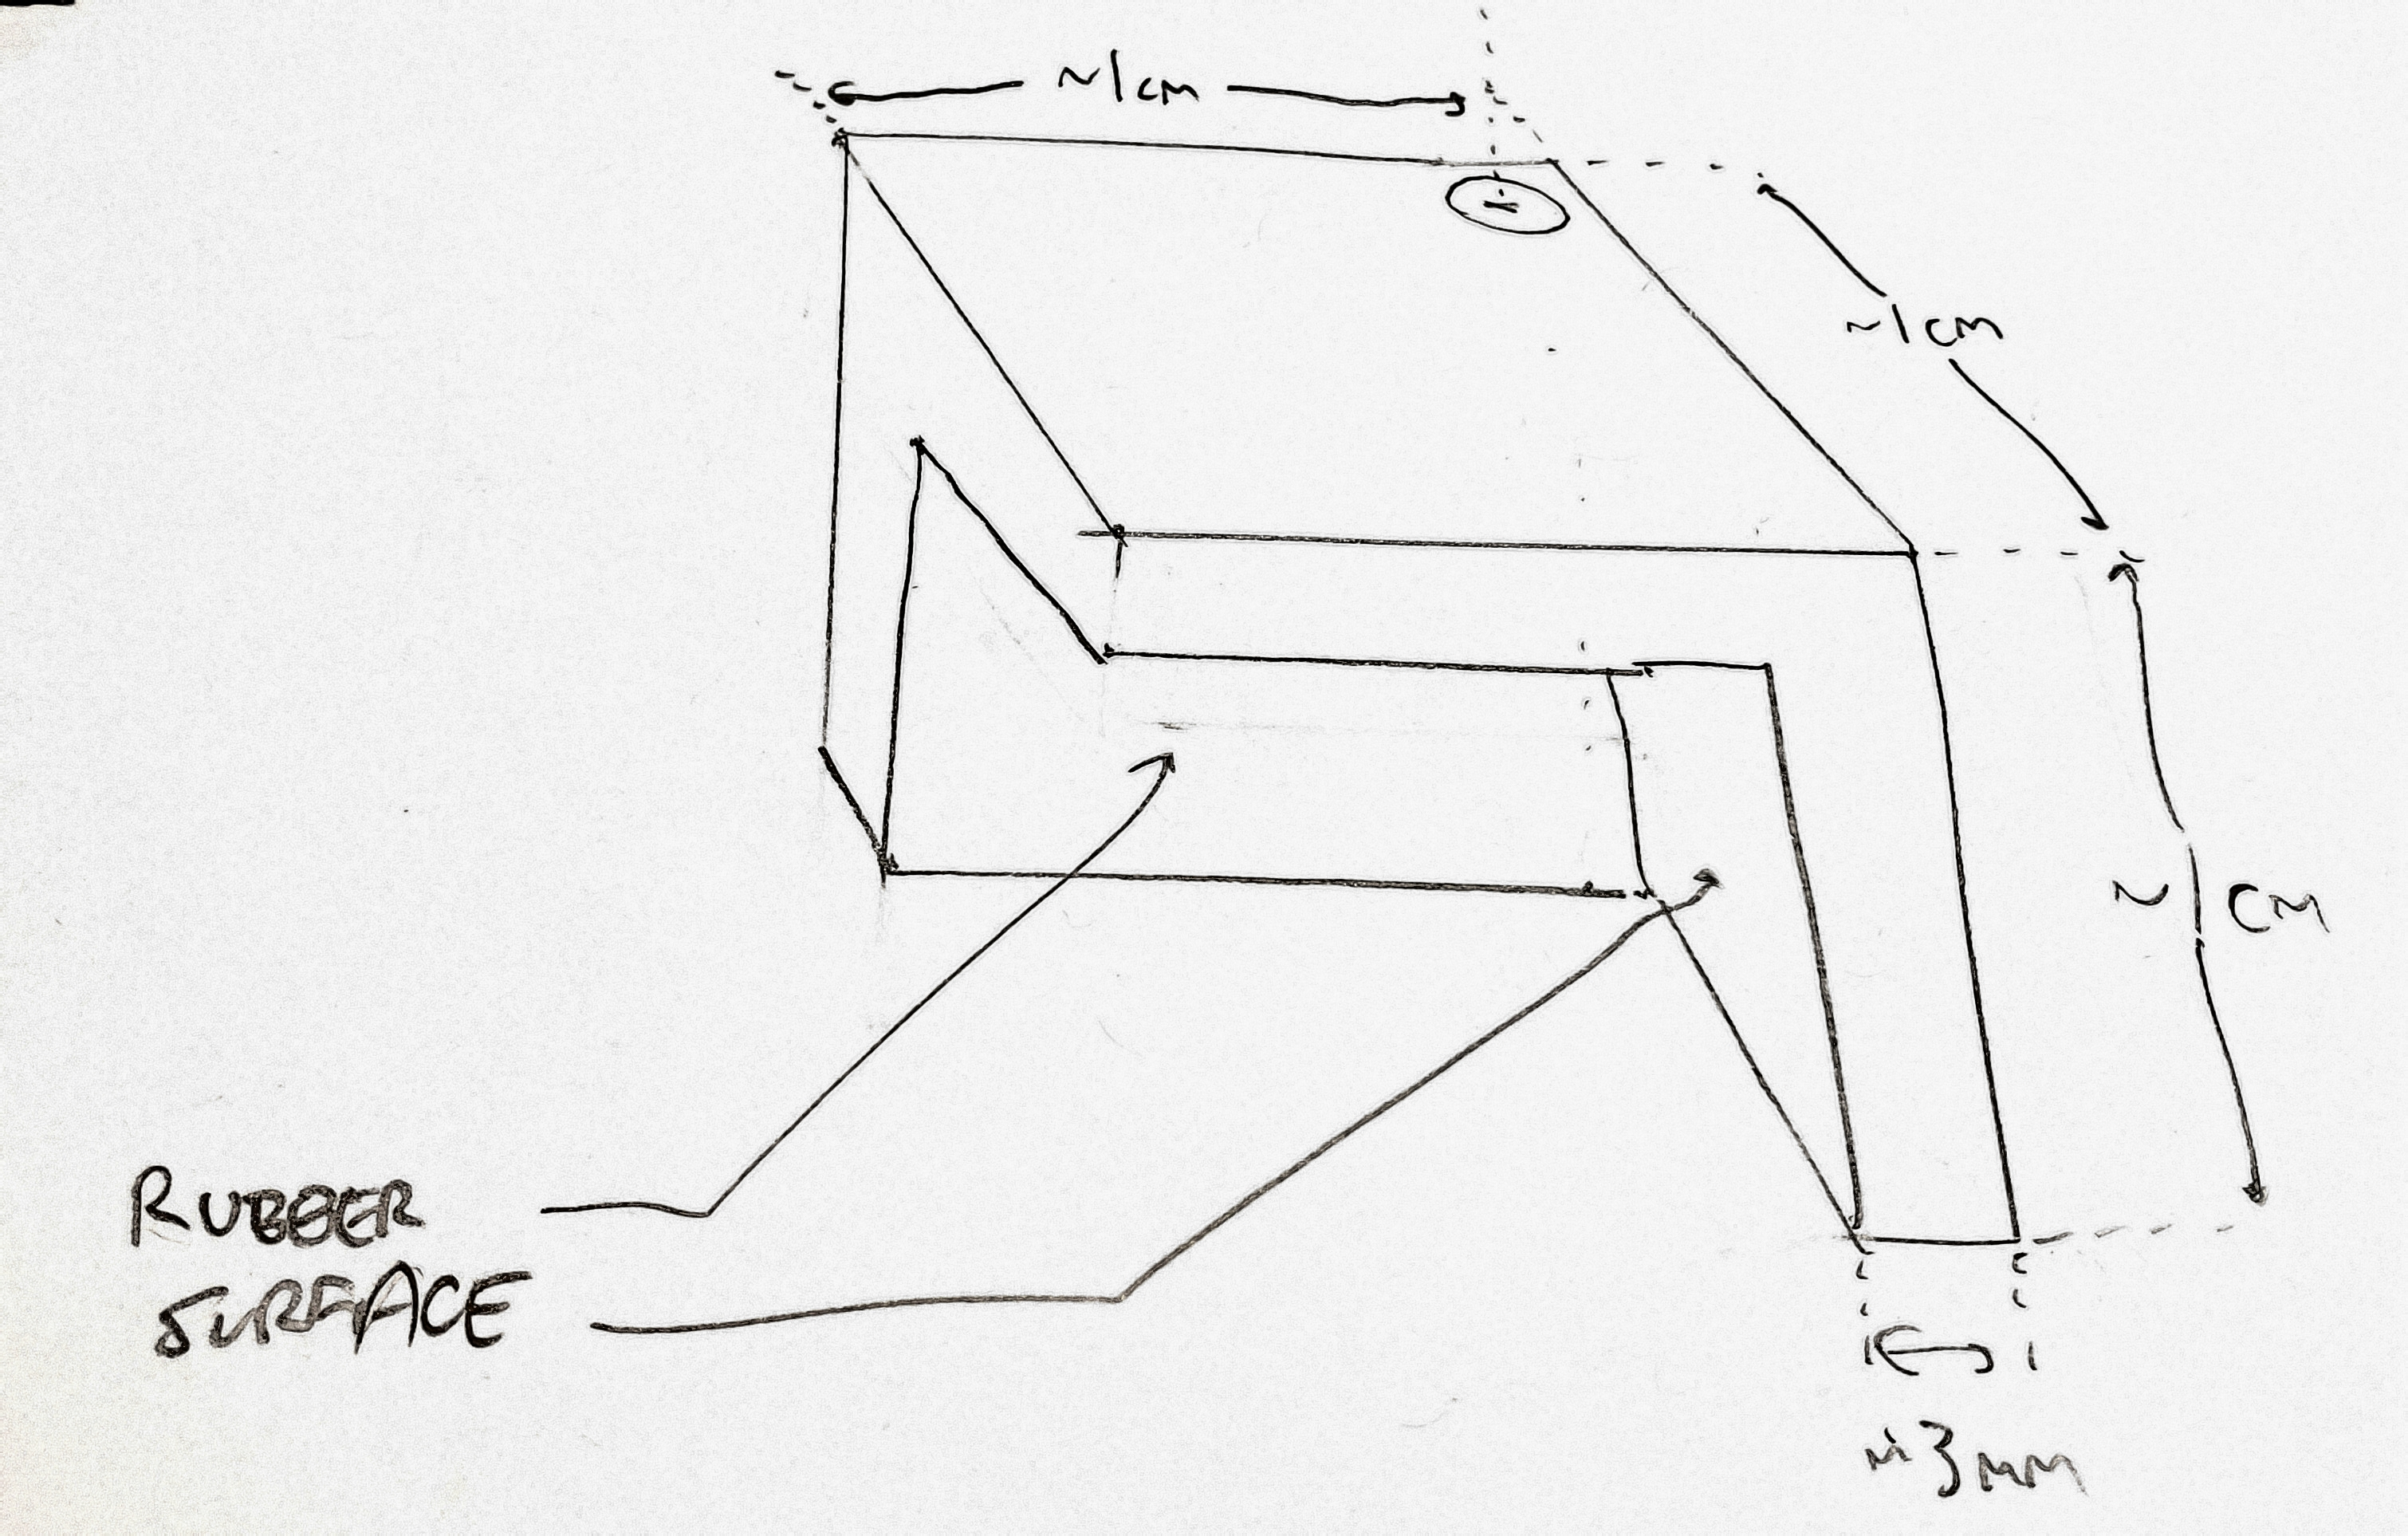
\includegraphics[width = 0.3 \textwidth]{PR2Images/CornerBracketPerspective.jpg}
				\caption{View of prospective design for corner clamp.}
				\label{fig:CornerClamp}
			\end{figure}

			\paragraph{Linear Travel}
			Because of the incongruities between effects pedals of different manufactures, a single set of bolt holes through the pedal plate will not suffice to accommodate most effects.  To solve this, the design will incorporate some combination of multiple holes in different locations and some slots through which the bolts can pass.
			
			To develop a flexible pattern of screw slots and holes, the dimension data collected from a sample of pedals from a Guitar Center retail location \cite{MyPedalData} was plotted in MATLAB, according to the dimension of the pedals' bottom plate screw holes, as seen in Figure \ref{fig:MATLABdimdata}.  The dimensions were grouped and a best fit line drawn for the main cluster.  This line was use to design a rapid prototype plate, seen in Figure \ref{fig:PlatePrototype}.  Fabricated using a laser cuter, the plate easily accommodates several average sized pedals that were easily available for this test.  Because of this success, this method of implementation of plate-pedal mechanical interface will be pursued for the first main prototype.

			\begin{figure}
				\centering
				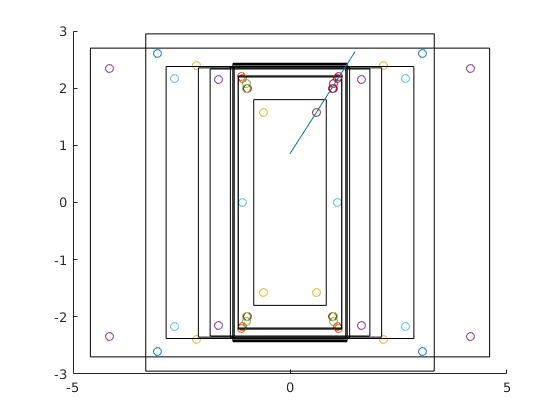
\includegraphics[width = 0.6\textwidth]{PR2Images/PedalBestFit.jpg}
				\caption{Plot of Common Guitar Pedals' Dimensions with Best Fit line through their bottom plate screw holes.}
				\label{fig:MATLABdimdata}
			\end{figure}

			\begin{figure}
				\centering
				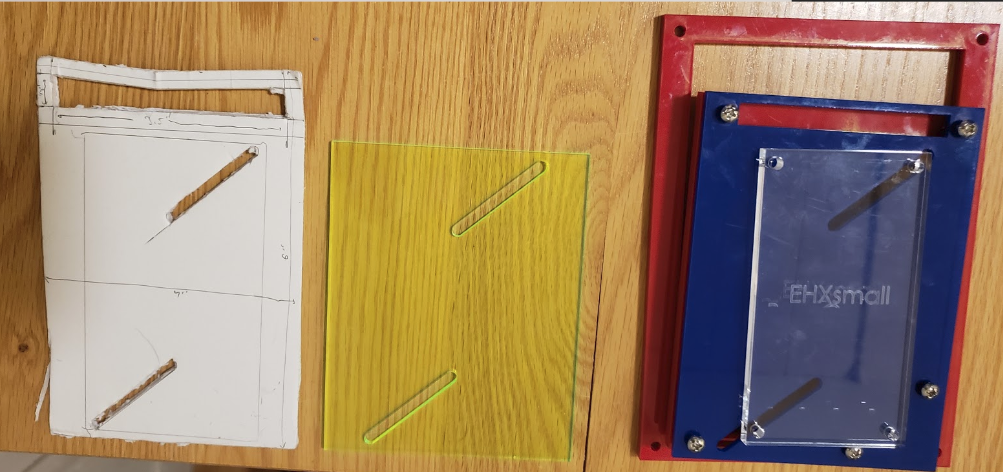
\includegraphics[width = 0.6\textwidth]{PR2Images/PlatePrototype}
				\caption{Prototypes of the pedal-plate attachment design.}
				\label{fig:PlatePrototype}
			\end{figure}

		\subsubsection{Plate Material}
		\label{Plate Material}
		The design of the plates was mainly informed by the incremental cost specification.  To keep the cost of producing a single plate low, the plate should be as simple as possible to fabricate.  As the plate requires a relatively large surface area, at minimum the size of an "average" guitar pedal, yet does not require for function significant thickness, the ideal form would be a single sheet of material.  The important design considerations for the material are that 
		\begin{itemize}
			\item the material must be rigid on the scale of a 5 x 5 inch plate.
			\item the material must be thin enough for the screws of the bottom enclosure plates to easily pass through (less than)
			\item the material must be easily cut with readily available CNC tools, namely a laser cutter or router.
			\item the material must be inexpensive.
			\item the material must not be easily bent or broken by drops or bumps.
		\end{itemize}
		The initial prototypes for the pedal-plate mounting design used 1/8" acrylic, cut with a laser cutter, because it was easily accessible.  However, acrylic can be brittle, so it is not a good choice for repeated handling by customers.  Another option was sheet aluminum, which has the benefit of being quite thin for its strength, making it easy for the pedal's screws to pass through.  A third option was to use the FR-4 grade glass epoxy resin used to make circuit boards.  In addition to being strong and lightweight, using this material allows for a simplification of the design.  Instead of sill needing to mount a circuit board to the main body of the plate, the circuit board can be the plate.  The physical layout of the screw slots can be cut at the same time as the board is shaped.  The wires to the plugs can escape directly from the surface of the board via a two position connector (such as the SWR201-NRTN-S02-SA-WH mated with a SWH201-NULN-S02-UU-WH from Sullins Connectors \cite{Sullinsdatasheet}). Other components such as switches used to select power can also be directly mounted and integrated with the board.  For its simplicity of design and manufacture, the first prototype will use this material and method for constructing the plates.

		\subsubsection{Plate-Receiver Electrical Connection Mechanism}
		\label{Pogo Pins}
		Moving signal and power between the plate and receiver is a vital task.  Though a number of guitar pedals offer processing of stereo signals, most are fully monophonic, requiring only one input and output connection.  In addition, because almost every pedal uses a single supply (non-bipolar) voltage, the simplest scheme for connecting a plate to its receiver requires only four connections: Power, Ground, Input (Send), and Output (Return).  This means that it is feasible to transfer the signal directly with individual physical connections, rather than some serial data protocol such as $\text{I}^2\text{s}$, which might be used if there were many inputs and outputs.  The use of "hard-wire" connections also keeps the signal "pure" by eliminating any unnecessary processing, which is an important consideration for marketing purposes.

		Making a consistent electric connection between the plate and receiver calls for some sort of spring loaded connector.  Unlike the connectors mentioned in Section \ref{Plate Material}, these connections are easy to break if desired, but still maintain good contact when connected.  They do not require the two surfaces to be exactly aligned, and they require only the single part to operate (instead of a matching male and female connector).  Figure \ref{fig:springloaded} shows some examples of spring loaded connectors.  On the left are connectors typically used to connect boards together within a product.  This class of spring connector is good for high pin count connections because of the large number of pins in a single unit, which are easy to manufacture cheaply.  For example, the 00-9258 type connector from AVX Corp costs \$0.77 for 8 electrodes from Digikey.  However, because these connectors are usually made for one time use when permanently assembling a product, they are not designed for repeated use.  For instance, the 00-9258 part is has a lifespan of just 50 cycles according to its datasheet \cite{AVX_00-9258_Datasheet}, which is certainly insufficient for this application.  For an order of magnitude estimate, each plate needs to be able to withstand 100 cycles per day for at least 1000 days (though the cycles/day is likely lower and the total days is likely higher).  This gives a ballpark estimate of 100,000 cycles minimum.

		\begin{figure}
			\centering
			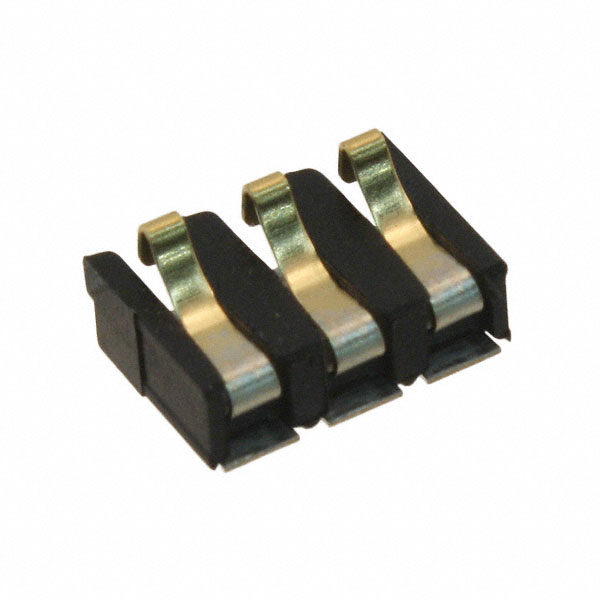
\includegraphics[width = 0.4\linewidth]{PR2Images/batteryconn}
			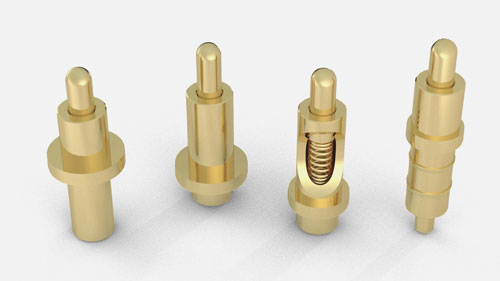
\includegraphics[width = 0.4\linewidth]{PR2Images/springpin.jpg}
			\label{fig:springloaded}
			\caption{Spring Loaded Connectors}
		\end{figure}

		In addition, because these connectors are designed for one time use, the order of connection does not matter.  However, for this application, there are some connections that must be "make-last, break-first," as will be described later.  This requires pins of different heights, which this type of multi-pin connector does not offer.  Instead, spring loaded pins like those on the right of Figure \ref{fig:springloaded} can be used.  This type of connector, sometimes known as a "Pogo Pin," includes a spring loaded plunger that sheaths into a sleeve.  These can be sourced through Digikey from Mill-Max, an industry standard manufacturer of milled connectors.  They have excellent electrical and mechanical characteristics, including 20m$\Omega$ contact resistance, minimum of 2 amp current rating, and a 1,000,000 cycle lifespan.  They come in a variety of lengths, though with less varied maximum strokes \cite{MillMax_025}.

		Using different length pins for different electrical connections allows some of these connections to be made or broken first.  In this case, most of the pins including signal and power will be of a standard height, but a shorter pin will be used to "mate-last, break-first" and will be used to ensure that the aforementioned connections are properly made before sending signal through to the plate.  In addition, a longer "mate-first, break-last" pin will be used as an inrush current limiter, as described in \cite{DesignforHotSwap}.

		Because these different pin heights are required, the design requires at least one of these spring loaded pins.  Their downside is in cost, as a pin like the costs about \$0.66 per pin.  Though the cost could be limited by using one of the multi-pin style connectors with a higher lifetime such as the Bourns 70AA series \cite{Bourns70AA_datasheet}, mixing the connection styles of the vertical-type spring loaded pins and the bending type multi-pin connectors would be difficult, in particular because of the difference in working heights.  The 0914 series spring loaded pins with the longest stroke length (for maximum height difference) are about 0.30" in height (before compression), while the uncompressed 70AA connector is 0.15" in height.  To mix these two types would require standoffs to adjust the uncompressed height, which determines the mate-order of the pins.  For simplicity, this prototype will use only pins from the 0914 series.

		Mill-Max offers many styles of spring loaded pins.  The first consideration was durability.  Though all of the pins examined are rated for 1,000,000 cycles \cite{MillMax_023}\cite{MillMax_025}, the through-hole versions likely offer better mechanical connection and stability with the circuit board, so these were preferred.  The next consideration was the ability to perform the mate-last, break-first operation, which requires as large a height differential as possible.  A large height differential will increase the time between the first and last pins making the connection, ensuring that the connections have been properly made and giving the circuit time to reach a steady state.  The pins are offered in short, standard, and long stroke lengths, which have maximum stroke depths of 0.039", 0.055", and 0.090" respectively. To achieve the longest time difference, the long stroke pins, series 0914 seem ideal.

		\begin{figure}
			\centering
			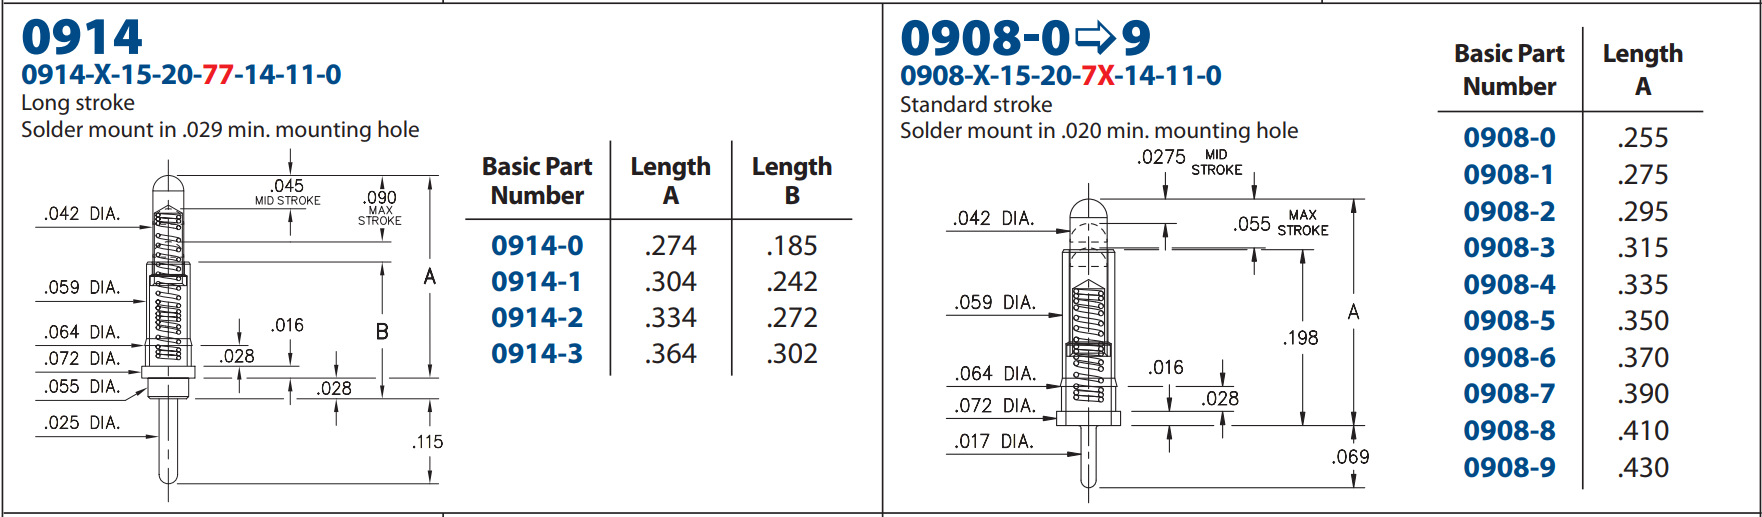
\includegraphics[width = \textwidth]{PR2Images/MillMaxSeries0914_0908.png}
			\caption{Mill Max Spring Pins, Through Hole, Long and Short Stroke}
			\label{fig:millmax0914_0908}
		\end{figure}

		As can be seen on the left in Figure \ref{fig:millmax0914_0908}, the B distance of the tallest pin determines the maximum travel of all of the pins, as this is the closest the plate can be to the surface of the receiver circuit board.  This means that 0914-0 and 0914-3 cannot be used together, as $B_3 = 0.302 == A_0 + 0.028 = 0.302$.  Only at 0914-3's maximum compression would 0914-0 make contact, so this will not work once the $\pm 0.006$ tolerances are taken into account.  However, any three consecutive pins will work together, which means choosing between using the 0914-0 and the 0914-3 (0914-1 and 0914-2 will be used in either case).  It turns out that the differences in length A any adjacent pins is 0.030", so the functional height difference between these two sets ({0, 1, 2} and {1, 2, 3}) are the same.  To reduce horizontal stress on the mounting, the shorter of the two options was chosen, as any tangential force on the end of the pin will result in less torque at the solder mount.  Thus the 0914-0 will be used for the make-last break first pins, the 0914-1 will be used for the standard input, output, and power pins, and the 0914-2 will be used for the inrush current limiting pin.

		\subsubsection{Plate Power Selection Method}
		In order to maximize the compatibility metric, the solution should be able to supply the most commonly required voltage and current supplies.  Though 9VDC is the de facto standard voltage supply \cite{MyPedalData}, there are a number of effects that accept 12 or 18 VDC, which can allow their amplifiers to have a higher headroom.  There are some other less common power supplies, such as 24 VDC for some older Electro Harmonix products, or 9 VAC for pedals like the Line 6 DL4 \cite{Line6DL4manual}, but these are rarer, so this prototype will focus on just the 9, 12, and 18 VDC supplies.

		In addition to varying electrical requirements, some pedals do not use the standard 2.1 mm power jack, with the center connector wired negative; a common alternative is a 2.5 mm jack with center positive connection.  Though this first prototype will focus on providing just the standard 2.1 mm center negative power, an extension to alternative connectors can be easily added via additional power supply cables which can plug into the plate via the same SWH201-NULN-S02-UU-WH type connector mentioned in Section \ref{Plate Material}.

		In order to supply power to the plate, there were two schemes to consider.  The first was a parallel supply, where all three voltages are connected to the plate at once, and the user who sets up the plate for a particular pedal can choose which connector to attach the power connector to.  This would allow a single voltage regulator for each supply voltage to be used.  However, this could run into issues of current draw, where many pedals could potentially draw more current than the voltage regulator can handle.  In addition, this would mean long traces in the main board carrying this voltage, which might experience a voltage drop due to the resistance of these traces.  Finally, this scheme requires two pogo pins per available voltage, one for the make-first inrush current limiting and another for the normal power supply.  Figure \ref{fig:parallelpowerschematic} shows an implementation of such a scheme.

		\begin{figure}
			\centering
			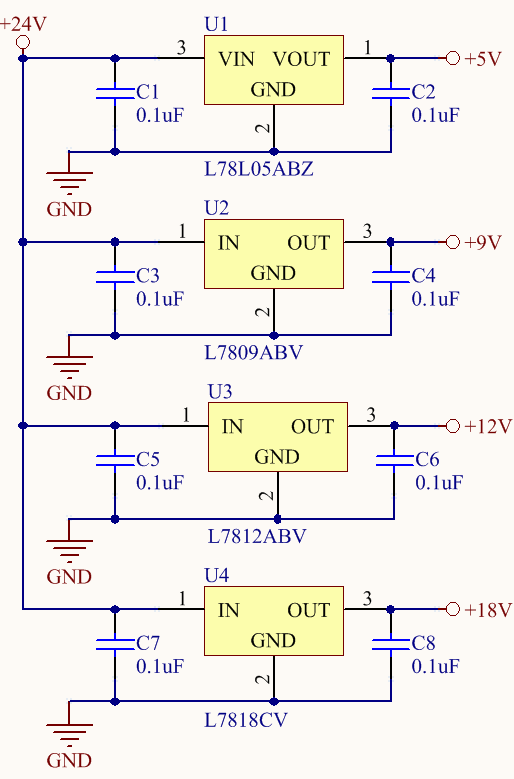
\includegraphics[width = 0.4\textwidth]{PR2Images/ParallelPowerSchematic.PNG}
			\caption{Power supply implementation where all voltages are available at all times.}
			\label{fig:parallelpowerschematic}
		\end{figure}

		The other option was to use a single voltage regulator for each plate, with a controllable output.  This eliminates concern over voltage drops between different receivers, and allows each receiver to draw as much current as a single regulator can supply.  For more than two power outputs, this method saves pogo pins, as only two pins are needed to supply the power (in addition to ground), though it does require several pins to communicate which voltage is desired for the current plate.  Instead of multiple connectors to allow the user to select the power connection, this method would use some switch, such as a two position DIP switch, to allow the user to set a binary value which can be decoded on the receiving end into the proper signals needed to control the adjustable voltage regulator.  As the pogo pins are fairly expensive (about \$0.66 each), reducing the number of pins is a good way to save on cost.

		The LM317 is a canonical adjustable voltage regulator, with its level set via a voltage divider (see datasheet section 8.2 for a typical application and design requirements \cite{LM317datasheet}).  The LM317 takes an input voltage between 1.25 and 37 V, preferably with $V_I - V_O > $ 3 V.  The difference $V_{OUT} - V_{ADJUST}$ is then kept at 1.25 V with a feedback circuit.  As shown in Figure \ref{fig:LM317_typicalapp}, this 1.25 V reference and $R_1$ then set the current through variable resistor $R_2$ ($I_{Adj}$ is negligible) which controls the output.  The $240 \Omega$ value for $R_1$ is a recommended value required to keep the output current high enough (over 3.5 mA) for a well regulated output.  The other diodes and capacitors are used to reduce ripple in the output.  Thus, $V_O$ can be given by

		\begin{align}
			V_O &= V_{REF}(1 + \frac{R_2}{R_1}) + I_{ADJ}R_2 \\
			&= 1.25 (1 + \frac{R_2}{240}) \quad \text{and} \\
			R_2 &= 240 \left( \frac{V_O}{1.25} - 1 \right) \\
			\label{eqn:LM317_R2}
		\end{align}

		However, a variable resistor for $R_2$ is not an easy method of setting the proper voltage for a user, because this would require individual tuning for each plate.  Instead, a set of switches is an easy mechanism for a user, who just needs to set the correct orientation of the switches.  A straightforward technique to use is switch in and out some additional resistors in parallel to a fixed $R_2$, as shown in Figure \ref{fig:adjustableregulatorschematic}.  Adding resistors in parallel reduces the effective resistance, reducing the output voltage, so the fixed $R_2$ should be calculated to set the maximum required output voltage, 18 VDC.  Using Equation \ref{eqn:LM317_R2} to calculate $R_2$ for an 18 V output gives $R_2 = 3.2 k\Omega$. The current through $R_1$ and consequently $R_2$ is $i_{R_1} = 1.25/240 = 5.2$ mA.  

		\begin{figure}
			\centering
			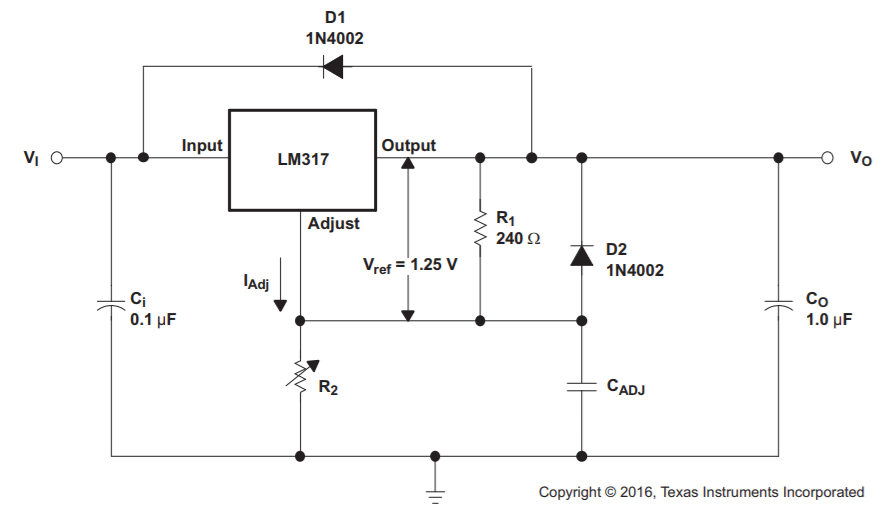
\includegraphics[width = 0.8\textwidth]{PR2Images/LM317_typicalapplication}
			\caption{Typical Application of LM317, from datasheet.}
			\label{fig:LM317_typicalapp}
		\end{figure}

		\begin{figure}
			\centering
			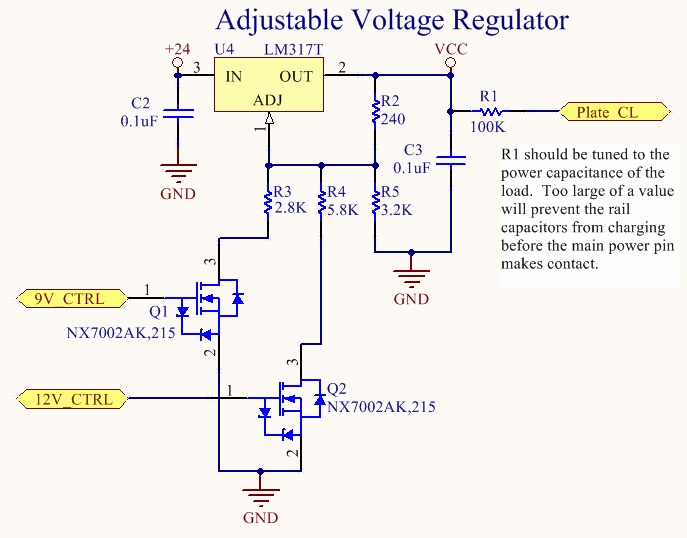
\includegraphics[width = 0.8\textwidth]{PR2Images/AdjustableRegulatorSchematic}
			\caption{MOSFET controlled adjustable regulator, with 9, 12, and 18 VDC selectable output.}
			\label{fig:adjustableregulatorschematic}
		\end{figure}

		MOSFETs are a good choice for this switch application because of their relatively low on-resistance $R_{DSon}$.  The cheapest type of MOSFET available from Digikey was the NX7002AK type, a ubiquitous single N-channel device \cite{NX7002AKdatasheet}.  With a maximum $V_{DS}$ of 60 V, a maximum $I_D$ of 190 mA for $V_{GS} = 10$ V at $25^o$ C, and a typical $R_{DSon}$ of $3.7 \Omega$ at $V_{GS}$ = 5V, this will work fine for this application, as would many standard MOSFETs.  In fact, because $R_{DSon}$ is on the order of Ohms while $R_2$ is on the order of Kiloohms, it can be neglected in the calculations for $R_3$ and $R_4$.

		For simplicity, let assume the MOSFET gate signals will not be turned on together, and that Q3 is used for a 9 V output while Q4 is used for a 12 V output, as in the following truth table:

		\begin{center}
		\begin{tabular}{c c|c}
			Q3 & Q4 & Output Voltage (V) \\
			\hline
			0 & 0 & 18 \\
			0 & 1 & 12 \\
			1 & 0 & 9 \\
			1 & 1 & X
		\end{tabular}
		\end{center}

		Because the MOSFET's on resistance can be ignored, solving for the $R_3$ when $Q_3$ is turned on so $R_3$ and $R_2$ are connected in parallel to ground gives

		\begin{align}
			R_3 || R_2 &= R_1 \left( \frac{V_O}{1.25} - 1 \right) = 240 \left( \frac{9}{1.25} - 1 \right) = 1488 \\
			R_3 &= \frac{1}{\frac{1}{R_3 || R_2} - \frac{1}{R_2}} = \frac{1}{\frac{1}{1488} - \frac{1}{3200}} = 2.8 k\Omega
		\end{align}

		Likewise, 

		\begin{align}
			R_4 || R_2 &= R_1 \left( \frac{V_O}{1.25} - 1 \right) = 240 \left( \frac{12}{1.25} - 1 \right) = 2064 \\
			R_4 &= \frac{1}{\frac{1}{R_4 || R_2} - \frac{1}{R_2}} = \frac{1}{\frac{1}{2064} - \frac{1}{3200}} = 5.8 k\Omega
		\end{align}

		Compute the power dissipated across these resistors to determine their necessary ratings.

		\begin{center}
		\begin{tabular}{c c|c}
			R ($k\Omega$) & V (V) & P (mW) \\
			\hline
			$R_1$ = 0.240 & 1.25 & 6.51 \\
			$R_2$ = 3.2 & 18 - 1.25 = 16.75 & 87.68 \\
			$R_3$ = 2.8 & 12 - 1.25 = 10.75 & 41.27 \\
			$R_4$ = 5.8 & 9 - 1.25 = 7.75 & 10.36
		\end{tabular}
		\end{center}

		Even with a 10\% safety margin, these resistors can all be 1/10 watt.

		\subsubsection{Receiver Plate-Removal Detection Method}
		To perform the automatic bypassing feature, the receiver must detect whether or not a plate has been inserted. Intuitively, the best way to do this seemed to be to use some of the same type of electrodes used to make connection between the plate and the receiver for signal and power.  This can be accomplished by using this extra detection pin as an SPST switch: when no plate is inserted, the switch is open, and when a plate is inserted, the switch closes.  This can signal some logic circuitry to activate the relay.

		To reduce transients that could result from suddenly connecting a plate and allowing the signal to flow before all of the necessary connections (Power, Ground, Input, and Output) are made, the receiver should wait to switch the relay from bypass to active until it is confident that all of the pins have made their connections.  This delay first relies on the bounce times of the pogo pins; like any mechanical switch, they will likely have some bounces or other irregularities in their switching, and one learning goal of the first prototype is to characterize this bounce.  To give an improved signal, the pin used to make this detection SPST switch will be set to "make-last, break-first," which will ensure that the other pins have already made first contact with the plate.  This is reflected in the choice of spring loaded pins described in section \ref{Pogo Pins}.  Assuming a 2 ft/s rate of descent (a high estimate) and the difference in height between the main signal connection pins and this make-last/break-first detection pin, there will be a $(0.030 in)/(24 in/s) = 1.33 ms$ difference.  Though this is likely not enough time to ensure the pogo-pins have stopped bouncing, the debouncing circuit block can and will increase this time delay before the signal to switch the relay is sent.  This time delay will need to be tuned to the specific bounce time of the pogo pins.

		To further ensure that the detect pin is the last to make contact, a second instance should be added for robustness against plates that are not inserted exactly vertically.  Assuming that the electrodes are aligned linearly, placing one detect electrode on each end of the line will ensure that both cannot make contact with the plate before the rest of the pins.  Thus, only when both electrodes have made contact should the relay be triggered.  Conversely, the relay should reset to bypass the plate when either of the electrodes break their connections.  This can be written as a boolean equation, where $A$ and $B$ are the status of the two detect electrodes (0 is disconnected, 1 is connected), and $R$ is the status of the relay, where 0 is plate-bypass and 1 is plate-active:

		\begin{align}
			R = A \cdot B
		\end{align}

		To reduce the number of pogo pins needed for this detection method, these detect pins will connect to ground, rather than 5 V, eliminating the need for an additional 5 V electrode to the plate.  Thus, these logic inputs will be active low: when a plate is inserted, the output of the switch will be 0 V, and when the plate is removed the output will be pulled up to 5 V via a pullup resistor on the receiver, shown in Figure \ref{fig:PlateDetectSwitch}.  Because of this, the A and B signals are given as their complements, and a NOR gate should be used instead of an AND.  

		\begin{figure}
			\centering
			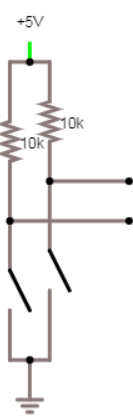
\includegraphics[width = 0.1 \textwidth]{PR2Images/PlateDetectSwitch}
			\caption{The spring loaded pins act as an SPST switch.  To reduce the necessary pins, they will connect the circuit to ground when the plate is in contact with the receiver, otherwise the pullup resistors will keep the signal high.}
			\label{fig:PlateDetectSwitch}
		\end{figure}

		On the insert transition the limiting factor on switching time (from bypassed to active) is on the order of 100 ms, the detectability threshold for visual-sound delay \cite{Timing}, which should not pose an issue with the switch debounce, logic, and relay switch times (~20 ms + ~0.1 ms + 2 ms = 22 ms \cite{EA2datasheet}).  However, the removal transition is limited by the time between the first detect electrode losing contact and the signal or power pins losing contact, which could cause transients in the output if the plate has not yet been bypassed.  By eliminating the switch debounce mechanism for this transition, the switch time can be lowered to approximately the operate time of the relay, which is about 2 ms.  This is quite close to the 1.33 ms estimate of the available window between the detect pin and the signal/power pins disconnecting.  As the estimate for this time difference is based on an order of magnitude type approximation, it is possible that there will be no issue, and no mitigation techniques need to be added.  A simple mitigation would be some transistor to pull the output to ground quickly (before the relay can be activated) so that any transients would be muted until the relay can successfully switch.  Because this would add complexity if not needed, this first prototype will proceed without this feature.

		\subsubsection{Receiver Bypass Mechanism}
		The primary function of the entire solution is to automatically bypass any receivers that do not currently have a plate inserted, so the choice of switching element is a key part of the design.  The basic choice here was between solid state analog switches or electromechanical relays.  The major design considerations for this choice are the signal to noise ratio, and the frequency response of the switching element.

		
		The initial value expected for the signal to noise ratio for an electric guitar was near 120 dBV.  Guitar pickups convert the mechanical energy of the vibrating strings to electrical energy via a coil of wire.  When the string vibrates in the magnetic field of a permanent magnet situated underneath, current is induced in the coil.  In an ideal environment, there should be little source of self noise because of the passive simplicity of this device, so any noise in the guitar signal is a result of the environment.  As such, the signal to noise ratio of a guitar can vary significantly based on the guitar's environment.  For example, guitar pickups are well known for their susceptibility to 60Hz line noise.  Therefore, the measured 90dBV signal to noise ratio should be taken as a minimum value, with 100dBV or more preferable.

		While solid state switches are more size, cost, and power efficient than mechanical relays, they may not have adequate signal to noise specifications, as well as crosstalk between channels on the same chip.  For example,the MT8808 Analog Switch Array \cite{Zarlink:MT8808} lists no specification on the device's signal to noise ratio, though it does boast a reasonable -90dB crosstalk between any channels for a 10kHz input with a $600 \Omega$ load.  The feed-through when a channel is off is listed as -95dB though, which is does not far exceed the minimum measured value for guitar signal to noise ratio, which could be an issue.  On the other hand, relay bypassing utilizing mechanical switches has no issues with signal to noise ratio, which would make it suitable for use in this project.

		As a minimum, the system should accommodate signals across the full range of human hearing, which is typically noted as 20Hz - 20kHz.  While this is the minimum acceptable range, there should also be allowance for lower and higher frequencies, which when used as input to a distortion effect can create inter-modulation distortion with frequencies in the audio range.  Neither of these ranges will be an issue however.  In the case that switching is accomplished with a solid state device, these are designed for frequency responses up to the tens of MHz range (the MT8808 has a 3dB frequency response of 45MHz), which is far greater than required.  If mechanical relays are used, there will likewise be no issues with frequency response in the audio range.
		
		

		These considerations suggest a preference for using mechanical relays despite their costs.  An additional reason is some of the interactions between the circuits on the guitar and in the first engaged pedal.  As mentioned above, the guitar pickup is made from a coil of wire, typically about 42 AWG with thousands of turns around a 6 inch or so circumference bobbin \cite{StewMacpickups}.  This long thin wire produces a DC resistance on the order of $10k\Omega$, which itself is quite a high output impedance, and the inductance and some parasitic capacitances from within the pickup will result in a frequency dependent output impedance with the potential to interact with a connected circuit block with sufficiently low input impedance.  In addition, the position of the guitar's volume potentiometer can affect the output impedance (see Figure \ref{fig:guitarpickupmodel} for a model of a guitar pickup and volume control circuit).  There are a number of guitar pedals known for their interaction with the guitar's volume knob; one of the best known is the Fuzz Face, first released in 1966 by Arbitrer Electronics \cite{FuzzFace}.  Following the same calculations as \cite{FuzzFace}, the input impedance to this pedal is about $8k\Omega$.  This does not follow the rule of thumb suggesting the input impedance should be an order of magnitude greater than the output impedance of the previous circuit stage, which means that there will be interactions between the guitar and this pedal.

		\begin{figure}
			\centering
			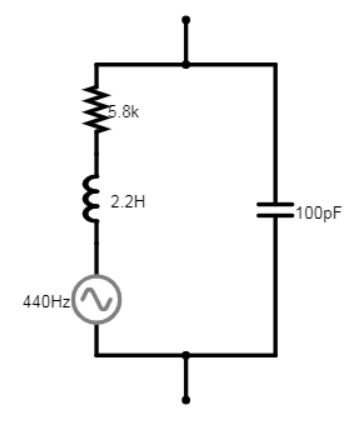
\includegraphics[width = 0.3\textwidth]{PR2Images/GuitarPickupModel}
			\caption{Model of guitar circuit.  These values are highly dependent on the particular pickups.  The potentiometer is either 250k or 500k.}
			\label{fig:guitarpickupmodel}
		\end{figure}

		Whether or not these interactions are good or bad, they have an undeniable effect on the sound and feel of playing the guitar through this pedal.  Inserting a buffer, including a solid state switch, between these circuit elements would destroy this interaction, and thus would prevent the solution from being an effect tool for comparing different pedals.  Therefore, the signal path should pass through no buffers when all receivers are bypassed, and electromechanical relays should be used to perform the switching.

		Because all of the signals being switched are low power, the relay can be in the "Low Signal Relays" category.  The cheapest available relay from Mouser was the EC2-12NJ from Kemet, a 12 V, 2 A, non-latching DPDT switch for \$1.69 each.  The DPDT type switch is preferable because only one package is required to perform the bypass switching per receiver.  The 12 V coil voltage requires less current (11 mA) than the 5 V coil which is also readily available (28 mA) \cite{EC2datasheet}.  The non-latching control makes for a very simple control circuit.  One issue with this though is that whenever the relay is activated, there is a constant 140 mW power dissipation required.  Though power is not a top priority, it would be beneficial to save power where possible, so a latching relay would be preferable in this aspect.  In addition, the datasheet claims that organic gases can build up inside the relay if the coil temperature rises due to long periods of activation current, which can result in faulty contacts \cite{EA2datasheet}, which could be solved through the use of a latching relay.  The EA2-5SNJ is available for just 9 cents more, and features a 5 V coil.  Although the lower voltage coil will draw more current when it is on, the relay needs be turned on only when being switched, so there is an overall savings in this regard.

		The EA2-5SNJ is a Form C type relay, which means that the DPDT switch operates break-before-make, ideal for this type of audio switching.  The device is a single-coil latch, where the coil is energized in one polarity to set the switch to one position, and is energized in the opposite polarity to set the switch to the other position.  This calls for an H-bridge style driver.

		\begin{figure}
			\centering
			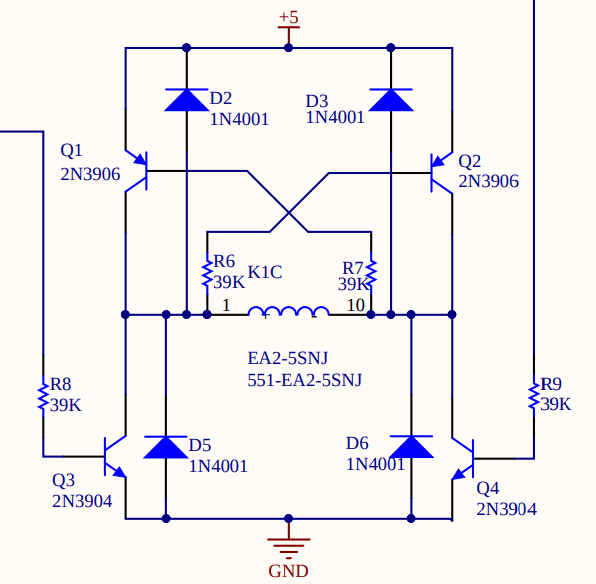
\includegraphics[width = 0.6\textwidth]{PR2Images/DiscreteHBridge.png}
			\caption{Discrete H Bridge implementation.  The inductor coil K1C load is the relay coil.}
			\label{fig:DiscreteHBridge}
		\end{figure}

		A standard discrete H bridge like the one shown in Figure \ref{fig:DiscreteHBridge} uses a quartet of transistors to power a load in either polarity or not at all.  When the two transistors in opposite corners (such as Q1 and Q4) are turned on at the same time, current flows through these transistors and the load, in this case the latching relay coil.  When it is time to set the relay's switch to the opposite position, the other two transistors are turned on instead and the load is energized with opposite polarity.  This implementation features garden-variety 3904/3906 type BJTs, which can supply plenty of current for the relay coil (just $5V/250\Omega = 20 mA$) \cite{EA2datasheet}\cite{2N3904datasheet}\cite{2N3906datasheet}, though these many other transistors would work.  D1-D4 are flyback diodes for the inductive relay coil.  To provide a load current of 

		\begin{align}
			i_{load} &= \frac{5V - V_{CE_4} - V_{CE_1}}{250 \Omega} = 18.4 mA
		\end{align}

		the base current of the transistors is related to the collector current by

		\begin{align}
			I_B &= \frac{I_C}{\beta}
		\end{align}

		The 2N3904 has a $\beta$ between 100 and 300 for a 10 mA $I_C$, so assuming $\beta = 200$ gives a required base current of

		\begin{align}
			I_B &= \frac{18.4mA}{200} = 92 \mu A \quad \text{and} \\
			R_2 &= 4.3V/92\mu A = 43 k\Omega
		\end{align}

		For a 10\% tolerance, use a $39k\Omega$ to ensure the transistor is turned fully on.

		A major issue with the H-bridge design is that both sets of transistors can never be turned on at the same time.  This would create a low impedance path from power to ground, cause high currents and potential damage to the circuit.  Though more of an issue in PWM motor control, a common application of the H-bridge, this "shoot-through" can occur when one set of transistors is switched on just as the other set is switched off.  Special protection should be taken to prevent such issues.

		For this reason, dedicated H-bridge driver ICs are offered.  One canonical example is the L298 dual H-bridge driver \cite{L298datasheet}.  It includes protection logic to prevent shoot-through and has enable inputs for each bridge.  This would be a good choice of driver, but for the price, which is about \$5 per chip from Digikey, which is more than the cost of the two relays it would be driving.  This is especially striking when considering that the cost of the MMBT3904 and MMBT3906 are \$0.10 and \$0.13 each.  For an integrated solution to be viable, it should not cost more than the relays it is driving.  Other options are the LV8548MC-AH \cite{LV8548MCdatasheet} and the LB1948MC \cite{LB1948MCdatasheet} from ON Semi.  These also have logic to prevent shoot through, and a thermal shutdown function to protect the chip.  Better yet, the LV8548MC-AH is available in a 10-SOIC package for \$1.33 each, putting the per-relay cost at just \$0.67.  This is on par with the cost of four of discrete transistors mentioned above.  Because the additional circuit protection justifies the use of this driver.

		Operation of the relay requires some logic to convert the plate detect signal to the proper signals required to switch the relay.  Although the EA2-5SNJ has a maximum operate time of 3 ms when driven at 100 mW (which is the nominal power applied to this 5V relay), the relay expects a pulse of more than 10 ms in duration \cite{EA2datasheet}.  As these should only be sent on the appropriate transition of the plate detect signal, an edge detector combined with a pulse generator should be used as the control logic, as shown in Figure \ref{fig:HBridgeCTRL_Block}.

		\begin{figure}
			\centering
			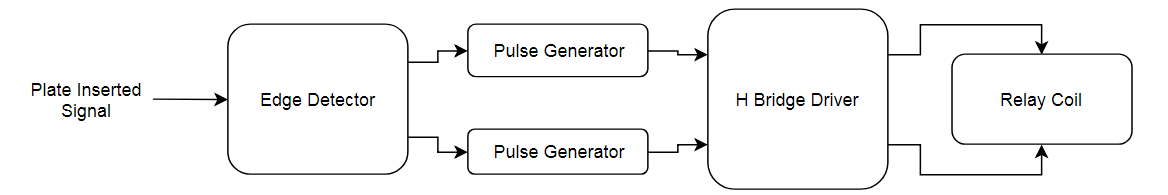
\includegraphics[width = \textwidth]{PR2Images/HBridgeCTRL_Block.PNG}
			\caption{Block Diagram depicting the control signals needed to drive the H bridge.}
			\label{fig:HBridgeCTRL_Block}
		\end{figure}

		The first implementation attempt first used a bidirectional edge detector circuit to generate the proper length pulse on any edge, followed by logic to determine the direction of the edge, such as in Figure \ref{fig:BidirectionalEdgeScheme}.  This required the use of an XOR gate in addition to typical NAND/NOR, and may be prone to race conditions resulting in both output signals going high at once.  For instance if C goes HIGH before D goes LOW, signal F and E could both asserted.  While this would not break the integrated H bridge solution, this is undesirable behavior, and the use of different types of gates would increase the cost and complexity of the BOM.

		\begin{figure}
			\centering
			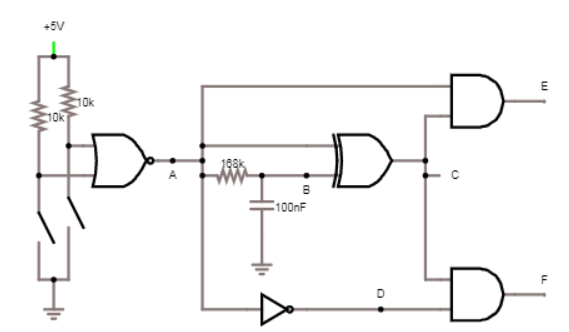
\includegraphics[width = 0.6\textwidth]{PR2Images/BidirectionalEdgeSchem.PNG}
			\caption{Edge detector and pulse generator.  This method first generate the necessary pulse on any edge, then extracts which edge (rising or falling) and sends the appropriate signal.}
			\label{fig:BidirectionalEdgeScheme}
		\end{figure}

		\begin{figure}
			\centering
			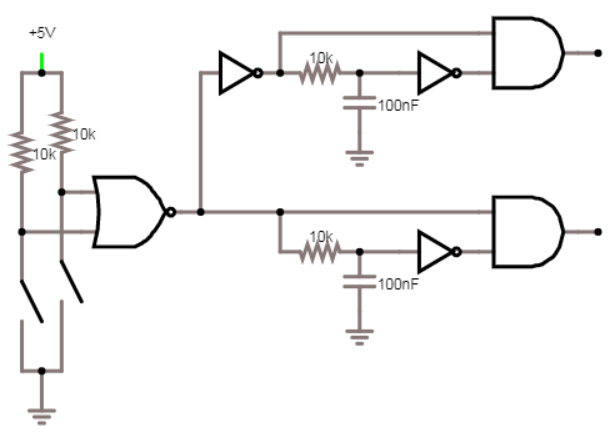
\includegraphics[width = 0.6\textwidth]{PR2Images/ParallelEdgeSchem.PNG}
			\caption{Edge detector and pulse generator.  This method applies one rising edge detector in parallel with one falling edge detector.  Note that the falling edge detector (top) is the just a rising edge detector with the input inverted.}
			\label{fig:RisingFallingParallel}
		\end{figure}

		\begin{figure}
			\centering
			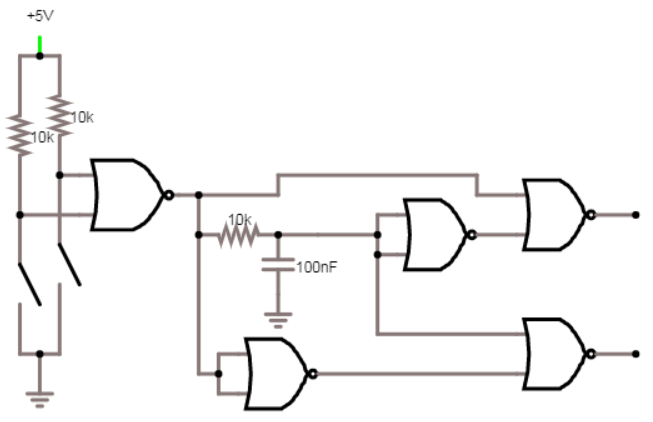
\includegraphics[width = 0.6\textwidth]{PR2Images/NOREdgeSchem.PNG}
			\caption{Edge detector and pulse generator.  This improved method combines the delay element of the previous one, and is implemented only with NOR gates, which helps with implementation.}
			\label{fig:ImprovedEdge}
		\end{figure}

		An alternative circuit is a rising edge detector in parallel with a falling edge detector, as shown in Figure \ref{fig:RisingFallingParallel}.  In this circuit, the signal is buffered then sent through an RC low pass filter to delay any edges and is inverted.  AND gates compare the delayed/inverted signal with the original and will output a pulse of proportional length to the RC constant of the filter if the two signals do not match.  This particular implementation would require 3 inverters, a buffer and two ANDs.  A simple optimization can combine the delay element into a single RC filter, which is fine if the pulse lengths for the two outputs can be the same length (in this case the requirement for both is $>$ 10 ms, so this is fine).  Figure \ref{fig:ImprovedEdge} demonstrates such a scheme.  In this implementation, the original signal, its delayed version, and their inverses are available to a pair of AND gates.  These inverters and gates should have Schmitt Trigger inputs to ensure a clean transition to generate the pulses.  With the signal labels from Figure \ref{fig:ImprovedEdge}, the function of the circuit can be reduced to a simple truth table

		\begin{center}
		\begin{tabular}{c c|c c}
			A & D & R & F \\
			\hline
			0 & 0 & 0 & 0 \\
			0 & 1 & 0 & 1 \\
			1 & 0 & 1 & 0 \\
			1 & 1 & 0 & 0
		\end{tabular}
		\end{center}

		This can be written as a set of boolean equations:

		\begin{align}
			R &= A \cdot \overline{D} \\
			F &= \overline{A} \cdot D
		\end{align}

		Because NOR/NAND gates are typically easier to implement and can also be used for the inverters, DeMorgan's Theorem can be used to convert these to their complimentary equivalents:

		\begin{align}
			R &= A \cdot \overline{D} = \overline{\overline{A} + D}\\
			F &= \overline{A} \cdot D = \overline{D + \overline{A}}
		\end{align}

		which can be implemented solely with NOR gates.  This is a perfect application of a quad, two input NOR gate such as the SN74HC7002 with Schmitt Trigger inputs \cite{SN74HC7002datasheet}.

		As the minimum pulse length to drive the relay is 10 ms, the pulse generate should aim for a longer pulse, perhaps 20 ms, to ensure the relay has been set to the correct position.  To determine the RC constant necessary to generate this pulse, consider the $V_{th}$ parameters of the SN74HC7002.  At $V_{CC} = 4.5V$, the positive going threshold voltage is at minimum 1.55 V \cite{SN74HC7002datasheet}, which is the case where the shortest pulse would be produced on a positive edge.  Solving the equation for RC capacitive charging gives

		\begin{align}
			RC &= \frac{-t}{\ln\left( 1 - \frac{V_{th}}{V} \right)} = \frac{-20ms}{\ln\left( 1 - \frac{1.55V}{5V} \right)} = 0.0539 s
		\end{align}

		so plugging in $C = 1 \mu F$ gives $R = 53.9 k\Omega$.  On the other hand, the maximum threshold voltage for a negative going transition is 2.54 V.  These $R, C$ values give a pulse time of 

		\begin{align}
			t  = - RC\ln\left( \frac{V_C}{V_0} \right) = -(53.9 k\Omega)(1 \mu F) \ln\left(\frac{2.54V}{5V} \right) = 36.5 ms
		\end{align}

		which is sufficient, though a slightly lower RC constant could reduce the excess pulse length.

		A full subsystem schematic of the receiver thus far is attached at the end of the document.  As implemented, the circuit uses 5 NOR gates, which poses a gate optimization problem, as this is just one more than a standard quad gate chip.  Unfortunately, the SN74HC7002, which is one of the only NOR gate ICs with a Schmitt Trigger input that will work with 5V, costs \$2.75 per chip.  To get around this cost, it would be possible to use an external Schmitt Trigger Inverter such as a 74AHCT14 type \cite{74HCT14datasheet}, which can be had for \$0.37 per chip, in conjunction with a non-Schmitt Trigger NOR gate, such as the 74AHCT02 \cite{74AHCT02datasheet}, which is just \$0.35 each.

		However, at this point, it may be cheaper and easier to use a microcontroller to perform this logic.  The obvious benefits of a microcontroller are:
		
		\begin{itemize}
			\item Reduced parts count: no need for external logic chips
			\item Can implement more complex logic, such as on board assurance that both H-bridge signals will not be on simultaneously
			\item Programmable debouncing of plate-detect pins
			\item Programmable pulse length for H-bridge driver
			\item Can also be used to control the adjustable power supply
		\end{itemize}

		Particularly because of the unknowns of the bounce characteristics of the pogo pins, the benefit of being able to easily adjust the debouncing is huge.

		To choose an appropriate microcontroller to determine if its cost will be worth it, the necessary features must be decided.  The first decision is how many receivers should be controlled by a single microcontroller.  The most straightforward replacement would be a one package per receiver.  This doesn't seem like the best option because any overhead required to implement the MCU would need to be repeated for each receiver.  The other extreme would be a single microcontroller for the entire main board.  This is not perfect either, as it would need a large number of GPIO, which is often supplied in difficult to assemble BGA type or other small packages.  In addition, a single centralized microcontroller would require long traces to reach the receivers, which could cause issues with signal integrity.  As the LV8548MC-AH are dual H-bridge drivers, a good compromise between these extremes is two receivers per microcontroller.  The microcontroller could be placed between two adjacent receivers to keep traces relatively short.

		To determine the number of GPIO required, count the number of I/O to this logic required per receiver:

		\begin{itemize}
			\item (2) Plate detect input pins
			\item (2) H-bridge driver outputs
			\item (2) Power Select outputs
			\item (2) Power Select inputs
		\end{itemize}

		This suggests a microcontroller with 16 GPIO is required for two receivers.  One cheap MCU available meeting this requirement is th ATTINY261A-MNR \cite{ATTINY261Adatasheet}, available in a 32-VQFN package for \$0.43.  A slightly larger package is the ATTINY40-SUR \cite{ATTINY40datasheet} in a 20-SOIC package for \$0.53.  The latter has 18 GPIO which could be useful for additional features later on, such as I2C communication between chips.  Although either of these or a number of others would work, the ATTINY40's extra GPIO package size make it a reasonable choice for this application, and actually reduces cost over the use of discrete logic components mentioned above.

		Now the function of the circuits described above can be implemented in code on the ATTINY40 and can be updated after fabrication.  A block diagram of the necessary functions is shown in Figure \ref{fig:MicroBlockDiagram}, along with a schematic showing the ATTINY40 interfacing with the peripherals at the end of the document.

		\begin{figure}
			\centering
			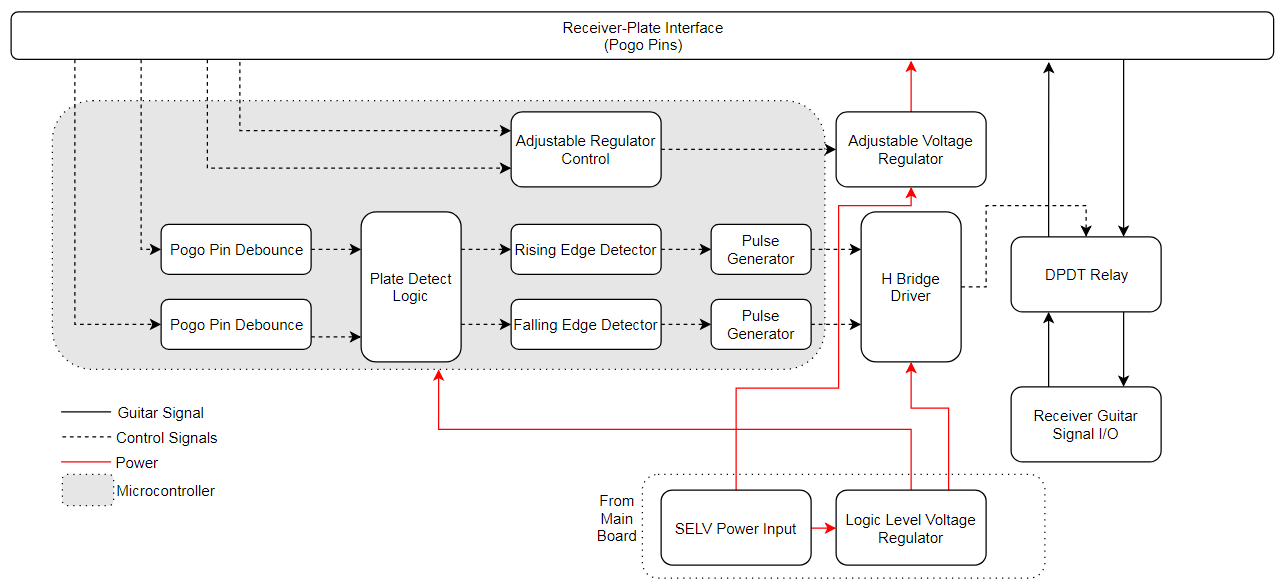
\includegraphics[width = \textwidth]{PR2Images/ReceiverBlockDiagramMCU.PNG}
			\caption{Receiver block diagram.  The blocks within the microcontroller are to be implemented in firmware.}
			\label{fig:MicroBlockDiagram}
		\end{figure}

	\color{black}



%%%%%%%%%%%%%%%%%%%%%%%%%%%%%%%%%%%%%%%%%%%%%%%%%%%%%%%%%%%%%%%%%%%%%%%%%%%%%%%%%%%%%%%%%%%%%%%%%%%%%%%%%%%%%%%%%%%%%%%%%%%%%%%%%%%%%%%%%%%%%%%%%%%%%%%%%%%%%%%%%%%%%%%%%%%%%%%%%%%%%%%%%%%%%%%%%%%%%%%%%%%%%%%
%%%%%%%%%%%%%%%%%%%%%%%%%%%%%%%%%%%%%%%%%%%%%%%%%%%%%%%%%%%%%%%%%%%%%%%%%%%%%%%%%%%%%%%%%%%%%%%%%%%%%%%%%%%%%%%%%%%%%%%%%%%%%%%%%%%%%%%%%%%%%%%%%%%%%%%%%%%%%%%%%%%%%%%%%%%%%%%%%%%%%%%%%%%%%%%%%%%%%%%%%%%%%%%
%%%%%%%%%%%%%%%%%%%%%%%%%%%%%%%%%%%%%%%%%%%%%%%%%%%%%%%%%%%%%%%%%%%%%%%%%%%%%%%%%%%%%%%%%%%%%%%%%%%%%%%%%%%%%%%%%%%%%%%%%%%%%%%%%%%%%%%%%%%%%%%%%%%%%%%%%%%%%%%%%%%%%%%%%%%%%%%%%%%%%%%%%%%%%%%%%%%%%%%%%%%%%%%
%%%%%%%%%%%%%%%%%%%%%%%%%%%%%%%%%%%%%%%%%%%%%%%%%%%%%%%%%%%%%%%%%%%%%%%%%%%%%%%%%%%%%%%%%%%%%%%%%%%%%%%%%%%%%%%%%%%%%%%%%%%%%%%%%%%%%%%%%%%%%%%%%%%%%%%%%%%%%%%%%%%%%%%%%%%%%%%%%%%%%%%%%%%%%%%%%%%%%%%%%%%%%%%
%%%%%%%%%%%%%%%%%%%%%%%%%%%%%%%%%%%%%%%%%%%%%%%%%%%%%%%%%%%%%%%%%%%%%%%%%%%%%%%%%%%%%%%%%%%%%%%%%%%%%%%%%%%%%%%%%%%%%%%%%%%%%%%%%%%%%%%%%%%%%%%%%%%%%%%%%%%%%%%%%%%%%%%%%%%%%%%%%%%%%%%%%%%%%%%%%%%%%%%%%%%%%%%
%%%%%%%%%%%%%%%%%%%%%%%%%%%%%%%%%%%%%%%%%%%%%%%%%%%%%%%%%%%%%%%%%%%%%%%%%%%%%%%%%%%%%%%%%%%%%%%%%%%%%%%%%%%%%%%%%%%%%%%%%%%%%%%%%%%%%%%%%%%%%%%%%%%%%%%%%%%%%%%%%%%%%%%%%%%%%%%%%%%%%%%%%%%%%%%%%%%%%%%%%%%%%%%







%%%%%%%%%%%%%%%%%%%%%%%%%%%%%%%%%%%%%%%%%%%%%%%%%%%%%%%%%%%%%%%%%%%%%%%%%%%%%%%%%%%%%%%%%%%%%%%%%%%%%%%%%%%%%%%%%%%%%%%%%%%%%%%%%%%%%%%%%%%%%%%%%%%%%%%%%%%%%%%%%%%%%%%%%%%%%%%%%%%%%%%%%%%%%%%%%%%%%%%%%%%%%%%
%%%%%%%%%%%%%%%%%%%%%%%%%%%%%%%%%%%%%%%%%%%%%%%%%%%%%%%%%%%%%%%%%%%%%%%%%%%%%%%%%%%%%%%%%%%%%%%%%%%%%%%%%%%%%%%%%%%%%%%%%%%%%%%%%%%%%%%%%%%%%%%%%%%%%%%%%%%%%%%%%%%%%%%%%%%%%%%%%%%%%%%%%%%%%%%%%%%%%%%%%%%%%%%
%%%%%%%%%%%%%%%%%%%%%%%%%%%%%%%%%%%%%%%%%%%%%%%%%%%%%%%%%%%%%%%%%%%%%%%%%%%%%%%%%%%%%%%%%%%%%%%%%%%%%%%%%%%%%%%%%%%%%%%%%%%%%%%%%%%%%%%%%%%%%%%%%%%%%%%%%%%%%%%%%%%%%%%%%%%%%%%%%%%%%%%%%%%%%%%%%%%%%%%%%%%%%%%
%%%%%%%%%%%%%%%%%%%%%%%%%%%%%%%%%%%%%%%%%%%%%%%%%%%%%%%%%%%%%%%%%%%%%%%%%%%%%%%%%%%%%%%%%%%%%%%%%%%%%%%%%%%%%%%%%%%%%%%%%%%%%%%%%%%%%%%%%%%%%%%%%%%%%%%%%%%%%%%%%%%%%%%%%%%%%%%%%%%%%%%%%%%%%%%%%%%%%%%%%%%%%%%
%%%%%%%%%%%%%%%%%%%%%%%%%%%%%%%%%%%%%%%%%%%%%%%%%%%%%%%%%%%%%%%%%%%%%%%%%%%%%%%%%%%%%%%%%%%%%%%%%%%%%%%%%%%%%%%%%%%%%%%%%%%%%%%%%%%%%%%%%%%%%%%%%%%%%%%%%%%%%%%%%%%%%%%%%%%%%%%%%%%%%%%%%%%%%%%%%%%%%%%%%%%%%%%
%%%%%%%%%%%%%%%%%%%%%%%%%%%%%%%%%%%%%%%%%%%%%%%%%%%%%%%%%%%%%%%%%%%%%%%%%%%%%%%%%%%%%%%%%%%%%%%%%%%%%%%%%%%%%%%%%%%%%%%%%%%%%%%%%%%%%%%%%%%%%%%%%%%%%%%%%%%%%%%%%%%%%%%%%%%%%%%%%%%%%%%%%%%%%%%%%%%%%%%%%%%%%%%
% \newpage
% \glsaddall
% \printglossarie
s% \newpage


% \newpage
% \bibliographystyle{plain}
% \bibliography{ThesisSources}

% \section{Appendix}

\section{Prototype Measurement Methods}
	The above documentation describes the design of the receiver prototype.  The electrical components including the circuit boards were fabricated using a milling machine.  The mechanical components including the enclosure were fabricated using a CNC router.  The code was written in C in Atmel Studio 7 and flashed to the microcontroller via the Ateml ICE in system programmer and debugger.  Testing the prototype to determine how well it matched the requirements began after fabrication was complete.

	\subsection{Swap Time}
	The success of this project in terms of a solution for improving the process of auditioning guitar pedals will be mostly a result of this measurement: how much time is saved swapping between pedals when using this system compared to the standard manual method?  The experiment used to measure this difference should simulate the expected operating conditions of the system.  In this case, a participant will conduct two tasks, and the time required to complete each of these tasks will be recorded.  For both tasks, the user begins with a guitar with its output connected through a single guitar pedal.  They must safely remove this guitar pedal from the signal chain, set it down in a defined location, touch a second location, then re-insert the pedal back into the signal chain.

	The first task is the control.  The guitar pedal is connected in the standard way, with an instrument cable connected from the output of the guitar to the input of the pedal.  The output of the pedal is connected to the input of a guitar amplifier.  The pedal is powered with a standard 9VDC wall wart adapter. The participant will be wearing the guitar (with a strap over their shoulder) to simulate real-world conditions.  To begin, the participant will have their left hand on the guitar's neck and their right hand touching the bridge (or the opposite in the case of a left-handed participant).  The pedal is set on a of standard height to mimic the environment of testing pedals in a guitar store, instead of on the floor.  After a countdown to let the participant know when to start, the timer will begin and the participant will quickly but accurately disconnect the pedal and place it on a marked rectangle on the table (shown in red).  The participant will, leaving the pedal in this marked rectangle, touch a second marker on the table (shown in blue).  This is to simulate the need to grab a second pedal without the experiment actually requiring the use of a second pedal.  After touching this blue marker, they will return the red rectangle to grab the pedal and re-insert it into the signal chain, making the input, output and power connections.  Then the participant will return their hands to the starting position on the guitar, which will signal the observer to stop the timer.  This measurement represents the time required to swap between pedals in the standard manual method.

	The second task is tests the hypothesis that the solution will decrease the swapping time.  This time the hot swapping unit is sitting on the table, with the instrument cable from the guitar plugged into its master input, and its master output connected to the input of a guitar amplifier.  The same pedal used for the control is connected to a plate (including all power and signal connections).  Before the task begins, this connected plate and pedal are inserted into one receiver on the hot swapping unit.  Again, the participant begins with their hands on the guitar.  When the timer starts, the participant removes the pedal and plate from the receiver, places it in the red rectangle, touches the blue marker, then retrieves the pedal and plate and reinserts it into the hot swap unit.  The timer stops when the participants hands both return to the guitar.  

	Both of these tasks should be repeated several of times for each participant, in this case three times, to ensure that a reliable measurement is recorded.  The test should also be performed with different pedals, especially ones of different size and with different I/O locations.  These pedals should be representative of the variety of pedals available.  The set of three pedals in Table \ref{tab:SwapTestPedals} should be representative of the range of products available that are compatible with the hot swapping system.  This means that each participant will perform nine trials of each task, totaling 18 trials.  Each trial should be no longer than one minute (and will likely be much less) so this is not an unreasonable number of tests per participant.  This experiment then should be conducted for a number of participants, at least ten, which should include both guitarists and non-guitarists alike.  Guitarists should have an easier time with the standard method, but comparing the measurements of non guitarists with guitarists should give an indication of how intuitive and simple the device is to use.  


	\begin{table}
	\begin{center}
	\begin{tabular}{ |c|p{8cm}| }
	\hline
	 Type Name & Description \\ 
	 \hline
	 $A$ & Mini sized pedal with side mounted jacks (similar to the TC Electronic Polytune 2) \\
	 $B$ & Standard sized pedal with top mounted jacks (similar to the EarthQuaker Devices Bit Commander) \\
	 $C$ & Oversizd pedal with side mounted jacks (similar to Electro Harmonix B9) \\
	 \hline
	\end{tabular}
	\caption{Set of three pedals used to represent the range of available products.}
	\label{tab:SwapTestPedals}
	\end{center}
	\end{table}

	Because this experiment requires some physical setup and scheduling for participants, it has not yet been conducted, but is planned for the week of February 18th after the PCBs are sent for fabrication.  For more details see the schedule near the end of this document.

	\subsection{Compatibility}
	The measurement for compatibility is not so much a matter of setting up a physical test but in determining which guitar pedals are likely to be available at music equipment retail locations and using the stated specifications for these to determine what ratio of them are compatible with the hot swapping device.  In this case, the list of common pedals was compiled by visiting brick and mortar music stores and taking stock of the products they had in stock.  Notably, the two Guitar Center locations in Boston were used to collect this data.  This list of available pedals which were photographed at the retail locations was entered into a spreadsheet.  Each entry was matched with a user manual and the available technical specifications were recorded.  These included:

	\begin{itemize}
		\item Physical Dimensions
		\item Range of Operating Voltages
		\item Required Current
		\item SNR
		\item Number and Description of I/O
		\item Input and Output Impedance
	\end{itemize}

	Data for more than 150 products from more than 25 companies were recorded.  This information was used to influence the design with the goal of accommodating the greatest number of available products.

	\subsection{Signal to Noise Ratio}
	The signal to noise ratio was measured for several different configurations of the unit.  An Audio Precision System One (AP) was used for all measurements.  This is a data acquisition device which can function as a test signal generator and a data recorder to measure the effect of the device under test.  The AP was connected to a computer via USB running its associated APWin software, allowing for control, processing, and visualization of the data.  For the SNR tests, one output of the AP was connected via a BNC-to-1/4" cable to the input of the device under test, and the output of the device under test was connected via a second BNC-to-1/4" cable to the corresponding input on the AP.  The AP's monitor output was connected to an oscilloscope to monitor the signal in real time.  To record the data, the AP measured the noise floor of the input and printed the value in dBu.  For each configuration being measured, the noise floor was captured for 20 trials.  The signal-to-noise ratio can then be computed from this noise floor measurement and the maximum supported signal for the device, which with a relay is almost arbitrarily large.

	The first test ($A$) was a control to understand the AP's own noise floor.  In this test, the output of the AP was connected directly to the input via a two foot BNC cable.  In this test, any noise recorded would be from the AP system itself, or noise picked up by this two foot coaxial cable, which limits the minimum detectable noise floor for the system under test.

	The second test ($B$) is of the prototype device with no power connected, and the signal switching relay on the receiver set to bypass.  Because the signal is mechanically connected directly from the input to output and no active circuitry is powered, this configuration should have the minimum noise floor among all measurements with the device under test.

	The third test ($C$) is of the prototype device with power connected and the signal switching relay on the receiver set to bypass.  In this case, the power supply is powering digital circuits on the same board as the analog signal, so a higher noise floor is expected.

	The fourth test ($D$) is of the prototype device with no power connected and the signal switching relay on the receiver set to send/receive.  In this case, a plate is inserted into the receiver with the plate's I/O connected to a guitar pedal which itself is in a hardwire bypass position, meaning that the plate's inputs and outputs are mechanically connected to each other.  This test will determine how much noise is picked up from the environment and the rest of the circuit board when the signal passes through the additional traces, pogo pins, cables, and jacks in the send/receive mode.

	These tests are summarized in Table \ref{tab:SNRtests}.

	\begin{table}
	\begin{center}
	\begin{tabular}{ |c p{5in}| }
	\hline
	Test ID & Description \\ 
	\hline
	$A$ & Measure test system noise.  AP output connect to AP input via 2' BNC cable. \\
	$B$ & Measure relay noise.  No power.   AP output connected to device under test (DUT) input, DUT set to bypass, DUT output connected to AP input. \\
	$C$ & Measure power supply noise.  Power connected.  AP output connected to DUT input, DUT set to bypass, DUT output connected to AP input. \\
	$D$ & Measure operation nose.  Power connected.   AP output connected to DUT input, DUT set to send/receive, plate inserted with hardwire bypass connection, DUT output connected to AP input.\\
   	\hline
	\end{tabular}
	\caption{Summary of SNR testing.  The AP System One was used to measure THD+N.}
	\label{tab:SNRtests}
	\end{center}
	\end{table}



	\subsection{Frequency Response}
	The frequency response of the unit was measured with the same Audio Precision device and setup as the signal to noise ratio.  For this test, the AP output a sine wave sweep over a set frequency range and recorded the response of the device under test.  The sweep consisted of 51 discrete frequencies ranging logarithmically from 10Hz to 30kHz, which covers the entire audio range with some margin.  Though the requirement for flat frequency response was specified down to DC, it is not possible to test arbitrarily low frequencies, so 10Hz was chosen as a suitable minimum bandwidth.  These test sine waves were output at 0 dBu, which is equivalent to 0.775 VRMS or 2.19 Vpp.  The AP then recorded the amplitude of the returning sine wave.  This entire process was automated, with each discrete frequency being tested and measured several times, thereby producing a reliable result.  This test was conducted on all of the configurations described in the SNR measurement section.  

	\subsection{Switching Time}
	When the receiver switches between the bypassed signal and the processed signal from a pedal, the switching time refers to the period of downtime between when the bypassed signal is present on the output and when the processed signal is present.  In the case of this implementation, this is the time required for the blade of the relay to move from one contact to the other.  This test was conducted by setting the AP to output a sine wave at a low fixed frequency, and connecting a pedal set to attenuate the signal.  The AP output was connected to the input of the device under test, and the output of the device under test was connected to the input of an oscilloscope.  The oscilloscope's trigger was set to a level just less than the peak voltage of the input sine wave.  The test is conducted by first inserting the pedal into the receiver so that the output is an attenuated version of the sine wave which does not cross the trigger threshold.  Then the oscilloscope trigger is set to single mode so that the oscilloscope will capture and hold the signals in the time adjacent to when the trigger was activated.  When the pedal is removed from the receiver, the signal output switches from the attenuated version that was processed with the pedal to the bypassed sine wave at a great enough amplitude to trigger the oscilloscope.  With the oscilloscope stopped, the vertical bars were aligned with the discontinuities resulting from the relay blade being switched (it is floating in between the contacts), and these bars are used to measure the time the relay is floating.  The image of this transition along with the switching time measurement was saved from the oscilloscope to an image file.  The switching time test was performed five times.

\section{Prototype Measurement Analysis}
	\subsection{Swap Time}
	Though the swap time test has not been conducted yet, once the data is collected, a one tailed paired T-test can be used to determine if the hot swapping device fulfilled its order of magnitude improvement goal.  The paired samples correspond to one participant's time required to complete each of the two tasks outlined in the Methods section.  Because each participant will conduct multiple trials of both tests, they will contribute multiple paired samples to the T-test.  Because the possible values recorded are continuous and the paired measurements are relatively randomly sampled (by choice of participant), the T-test should be reliable.

	\subsection{Compatibility}
	The data collected was analyzed using MATLAB.  First, the data was broken down by company, and each company was assigned a numerical ID.  The number of pedals available from each manufacturer was counted.  Then the data was further broken down by pedal enclosure category.  Generally, each manufacturer will design many of their products to fit in the same enclosure, which keeps their procurement and design process simpler.  This allows the pedals to be grouped by enclosure type, meaning that all pedals offered with the same enclosure will have the same external dimensions and be mechanically compatible with the hot swapping device if any one of them is compatible.  Each enclosure type was also given an ID number, and was labeled with the company who uses it and the number of products being offered by that company using this enclosure type.  This data was plotted using a stacked bar graph as seen in Figure \ref{fig:pedalsAvailable}, with the company ID numbers listed in Table \ref{tab:pedal_companies}.  Note for instance that Company 12 (Boss) offers more than thirty pedals, and the vast majority of these use the same variety use the same type of enclosure, meaning that compatibility with this type of enclosure is a greater priority than a lesser used one, such as the type used by Company 9 (ProCo).  Note that the plot only shows effects with their physical dimensions listed in the manual, which explains why J Rockett Audio, which had two products, has no bar on the graph.

	\begin{figure}
		\centering
		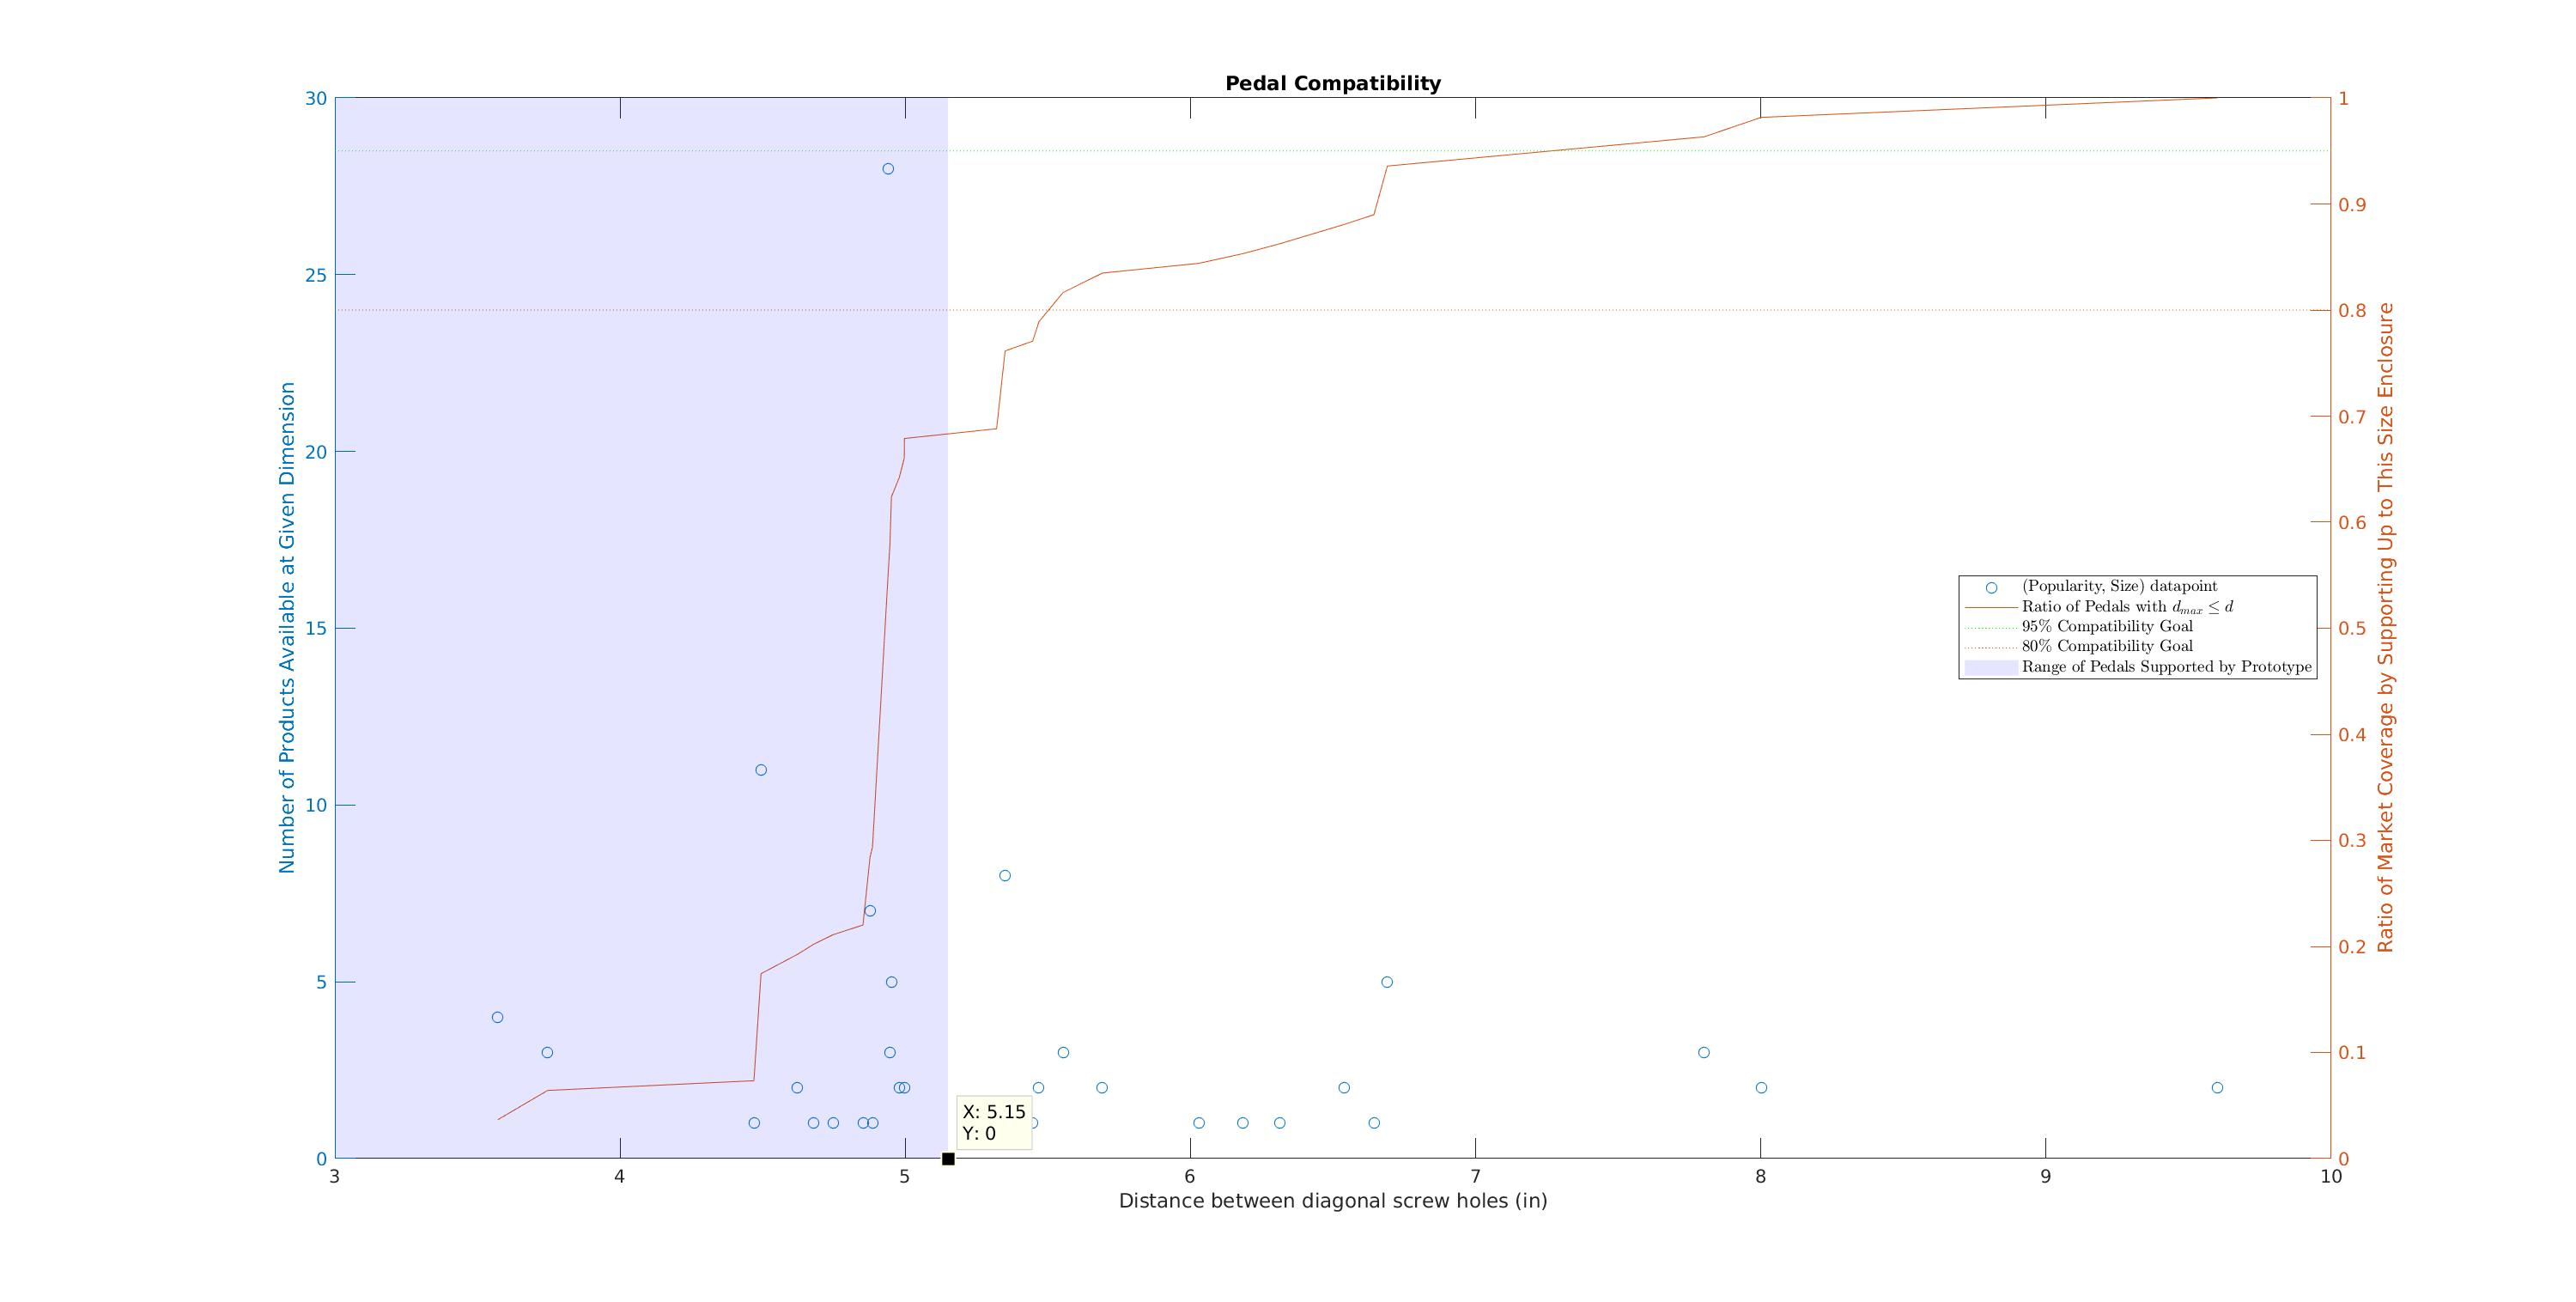
\includegraphics[width = 0.8\textwidth]{PR4Images/PedalsAvailable.jpg}
		\caption{Number of guitar pedals available by manufacturer ID.  The bars are divided vertically by the type of enclosure used, with the most popular enclosures on the bottom.}
		\label{fig:pedalsAvailable}
	\end{figure}


	\begin{table}
	\begin{center}
	\begin{tabular}{ |c c c| }
	\hline
	 Company Name & Company ID & Number of Products Available \\ 
	 \hline
	Seymour Duncan    &  1        &  4     \\
    BBE               &  2        &  1     \\
    J Rockett Audio   &  3        &  2     \\
    Tech 21           &  4        &  2     \\
    Ampeg             &  5        &  2     \\
    MXR               &  6        & 18     \\
    Korg              &  7        &  1     \\
    Fulltone          &  8        &  6     \\
    ProCo             &  9        &  1     \\
    Danelectro        & 10        &  3     \\
    Digitech          & 11        &  7     \\
    Boss              & 12        & 33     \\
    Eventide          & 13        &  1     \\
    Way Huge          & 14        &  2     \\
    Egnater           & 15        &  1     \\
    Line6             & 16        &  1     \\
    Fender            & 17        &  3     \\
    Voodoo Lab        & 18        &  1     \\
    EHX               & 19        & 26     \\
    Ibanez            & 20        &  5	   \\    
    Maxon             & 21        &  1     \\
    EarthQuaker       & 22        &  8     \\
    JHS               & 23        &  4     \\
    Keeley            & 24        &  5     \\
    TC Electronic     & 25        & 13     \\
   	\hline
	\end{tabular}
	\caption{List of guitar effects manufacturers and their associated ID numbers.}
	\label{tab:pedal_companies}
	\end{center}
	\end{table}

	To determine which pedals will be mechanically compatible, their dimensions were compared with the dimensions of the currently plate.  Because of the "opposite corners" mechanical connection technique where the screws from two of the pedal's corners are connected through the plate to make the mechanical connection, any pedal will fit if the distance between its opposite corners (less some factor to account for the positioning of the screws slightly inside the outer dimensions of the enclosure) is within the range permitted by the plate design.  The plate prototype can support pedals with a minimum screw hole distance of 2.5" and a maximum distance of 5.2".  Figure \ref{fig:pedalcompatibility} describes the compatibility of the plate prototype with the different pedals available.  The x axis represents the distance between opposite screw holes for a given enclosure.  The data points of the scatter plot represent each type of enclosure cataloged, positioned by this screw hole distance and by the number of different products available that use this same enclosure, which is shown on the left y axis. The line plot is the cumulative ratio of the products available with their screw hole distance less than the current $d$ value on the x axis out of the total number of pedals available.  Assume the plate can support all pedals up to a given dimension, this line can be used to determine the ratio of compatibility for the design.  The 80\% and 95\% goals are shown as horizontal lines.  The compatibility of the first prototype is depicted by the blue shaded region at left, which covers all screw hole distances up to 5.2".  The intersection of the rightmost boundary of this blue region with the line plot gives the current compatibility, which is just shy of 70\%.

	\begin{figure}
		\centering
		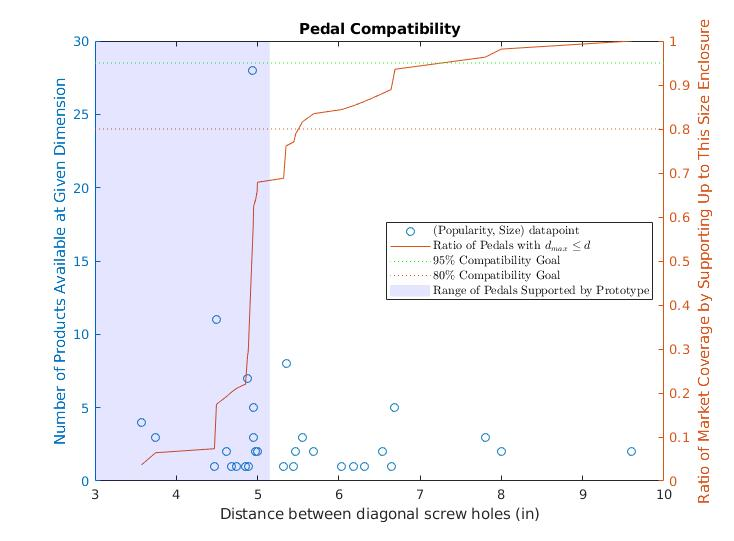
\includegraphics[width = \textwidth]{PR4Images/PEdalCompatibility.jpg}
		\caption{}
		\label{fig:pedalcompatibility}
	\end{figure}

	This plot can be used to improve the design of the plate to find a balance between increasing the size of the plate to improve compatibility while not wasting space.  For instance, there are two clusters in the x direction of pedals with screw hole distances less than 6" and 7", respectively.  Increasing the size of the plate to 6" would result in an 85\% compatibility ratio, which would meet the specifications.  This is a good trade-off of size versus compatibility.  In fact, increasing the plate size to 7" would allow the design to reach the 95\% goal.  However, if the plate size was increased enough to reach every single enclosure, the additional size would not add very much compatibility, so that would be a poor trade-off.

	Although the current prototype fails to meet either the 80\% or 95\% requirement, this is not a major issue.  The goal of the prototype was to test the hot-swapping features and get a sense for problems the plate might have.  With this groundwork in place, the plate size can be changed to fit requirements without much issue.

	\subsection{Signal to Noise Ratio}
	The data collected from the measurements is summarized in Table \ref{tab:SNRresults}.  Test $A$ shows the limits of observation with the Audio Precision measurement device.  Because the system has -107 dBu noise floor by itself, it will not be able to detect if the DUT has a lower noise floor.  This is an industry standard measurement device, so using this instead of a potentially lower noise one is reasonable.  In addition, the actual values obtained during this tests qualitatively seemed affected by quantization noise.  Only a handful of discrete values were recorded over the 20 trials for this test.  These measurements taken were of the noise floor, which is only one of the two values needed to compute the SNR.  The maximum signal level is also required.  This can be difficult to determine when relays are used, as the signal can be arbitrarily large up to the maximum isolation voltage of the relay, which could be in the 100s or 1000s of volts, which would skew the SNR.  A better value to use would be the maximum supply voltage the device makes available to pedals, 18V, as this is the largest expected signal for the receiver under normal circumstances.  In units of dBu, 18Vpp = 12.7279Vrms = 24.3136dBu.  Therefore, the SNR of the system is the absolute value of the mean measured THD+N value plus 24.3136.  These SNR values are also given in Table \ref{tab:SNRresults}

	Test $B$ shows the noise floor for the device with no power connected.  The mean noise was the same as test $A$, which shows that the relay is an excellent choice for signal integrity.

	Test $C$ shows the noise floor with the power connected.  Here the mean noise floor increased to -82 dBu, a three order of magnitude increase.  This is a result of the switching noise from the switching power supply being coupled onto the audio signal.  This noise is particularly problematic because it had a noticeable frequency component around 20kHz, which is just at the upper end of the audio spectrum, meaning that this noise could be heard through the speakers during use.  Although the resulting SNR does meet the 90dBu minimum requirement, it does not achieve the desired 120dBu requirement.  Therefore, effort should be taken to mitigate the resulting power supply noise.

	One simple solution for the power supply noise issue is the introduction of a common mode choke at the power input to the device.  The common mode choke performs a similar function to a pair of inductors connected in series with the power and ground lines respectively.  By limiting the change in current on these wires, the choke can reduce switching noise, even noise that is present on the system's ground.  To this end, an additional test $C'$ was performed with a choke connected between the switching power supply and the device's power input.  As can be seen, the noise floor reduced markedly, returning to near the limits of the AP measurements system.  

	Because the previous test successfully demonstrated the effectiveness of the choke in mitigating the power supply switching noise, the remaining test was modified to include the common mode choke, now labeled as test $D'$. The noise floor increased slightly over the bypassed mode, which makes sense as the audio signal now must travel through additional traces, wires, and components.  In addition, the guitar pedal power supply is also traveling through additional unshielded cables, all of which provides opportunity to pick up noise.  However, the noise floor is still very low, and meets the 120dBu requirement.  With the inclusion of the common mode choke, no changes must be made on this system to maintain the specified requirements.

	\begin{table}
	\begin{center}
	\begin{tabular}{ |c c c c| }
	\hline
	Test & Mean THD+N (dBu) & Variance (dBu) & SNR (dBu) \\ 
	 \hline
	$A$ & -106.9621   & 0.0178 	& 131.2757 \\
	$B$ & -106.8596   & 0.0157 	& 131.1732 \\
	$C$ &  -82.0101   & 0.1373  & 106.3237 \\
	$C'$ & -106.6603   & 0.1566 & 130.9740 \\
	$D'$ & -104.9962   & 0.0357 &  129.3098 \\
   	\hline
	\end{tabular}
	\caption{Results of SNR testing.  The AP System One was used to measure THD+N.}
	\label{tab:SNRresults}
	\end{center}
	\end{table}

	\subsection{Frequency Response}
	The frequency response measurement recorded data at 51 different frequencies, ranging logarithmically from 10 Hz to 30 kHz.  At each frequency, the AP sent a 0dBu sinusoid and measured the amplitude of the signal returned at its input.  The frequency response was measured with the hot swapping device in send/receive mode with the common mode choke in place to replicate expected operating conditions.  The results of the test are plotted in Figure \ref{fig:FRplot}.  As can be seen, the measured signal in blue was always measured with to have a smaller amplitude than the output reference signal in dashed black, which makes sense considering the analog signal path is passive, so only losses should be experienced.  Because this is the highest noise configuration with the longest signal trace length, these results should be taken as something of a worst case value.  The requirement for signal integrity was to keep the change in amplitude across the tested spectrum less than 0.1 dBu up or down, represented by the shaded blue region on the graph.  A successful device would keep the measured response within the shaded blue region, and as can be seen this device meets the requirement.  In fact it is only at the low range, around 12 Hz that the signal dips anywhere near the maximum offset.  Because 12 Hz is below the audio spectrum, this is not a very big issue.

	\begin{figure}
		\centering
		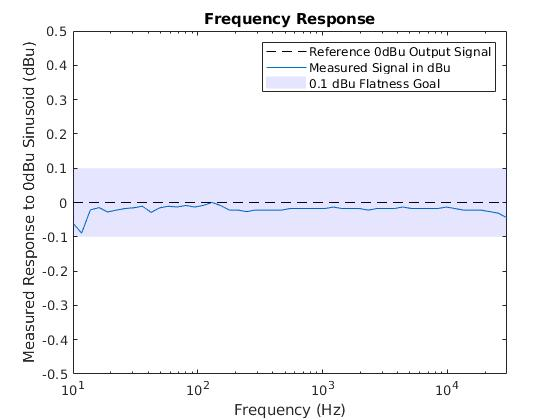
\includegraphics[width = 0.8\textwidth]{PR4Images/FRactive.jpg}\
		\caption{Frequency response of the receiver in active send/receive mode.}
		\label{fig:FRplot}
	\end{figure}

	\subsection{Switching Time}
	The switching time is the elapsed time between when the two signals are present at the output when the relay switches.  It was measured five times using the trigger of an oscilloscope.  The times measured were
	\begin{table}[H]
	\begin{center}
	\begin{tabular}{|c|c c c c c|c c|}
	\hline
	Trial & 1 & 2 & 3 & 4 & 5 & Mean & Variance \\
	Value ($\mu s$) & 350 & 400 & 400 & 420 & 436 & 401.2 & 1047.2 \\ 
	\hline
	\end{tabular}
	\caption{Measured relay switching times.}
	\end{center}
	\end{table}

	\begin{figure}
		\centering
		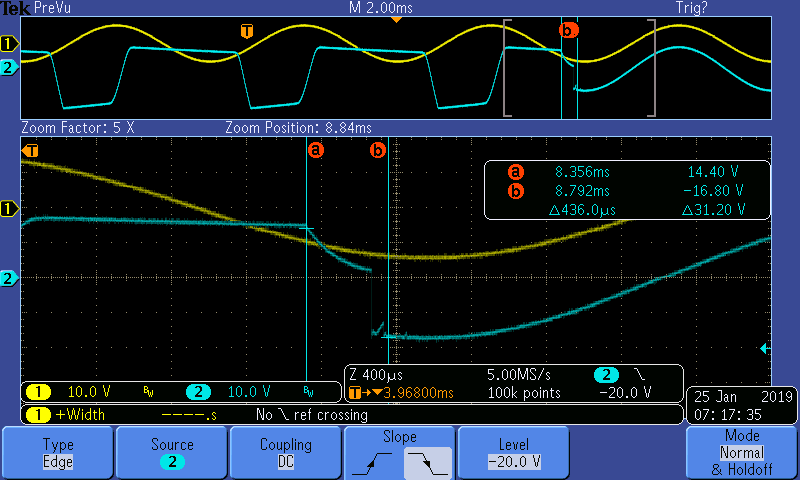
\includegraphics[width = 0.8\textwidth]{tekmeasurements/tek0004.png}\
		\caption{Oscilloscope capture of the signal switching event.  Note the vertical rulers used to measure the elapsed switching time.}
		\label{fig:relayswitching}
	\end{figure}

	Figure \ref{fig:relayswitching} shows one of the captured oscilloscope images of a switching event.  In this image, the yellow signal was the reference sinusoid connected the receiver's input.  The blue trace is the output of the receiver.  Before time $a$, the receiver is set to send/receive mode and the output signal is being clipped by a connected pedal. At time $a$, the relay blade breaks contact and is left floating.  It can be seen discharging to ground 300$\mu$s or so.  At around $a + 300\mu$s, the relay blade makes first contact with the other electrode, and the output is pulled down to the level of the sinusoid.  Just before time $b$ the relay blade bounces and the output again attempts to discharge back to ground before the blade stops bouncing and the output is fully connected to the sinusoid at time $b$.  Although there are very few samples, it was clear that they were more than an order of magnitude less than the requirement of 20 ms, so the precision of the measurement was not very important.  In addition to this quantitative testing, qualitative listening tests showed no perceived gap in the output, so this requirement is satisfied.

	\subsection{Transient}
	Transients resulting from signal switching can arise from two main sources.  The first is the system itself.  This could result from some microphonic components in the system picking up the mechanical vibrations when the relay blade moves between the contacts.  It could also result from the relatively large switching current driving the relay or other digital components coupling into the audio signal.  If instead a solid state analog switch had been used, the charge injection resulting from stray capacitances in the MOSFET devices could cause a shift in level, resulting a transient when switched \cite{ADI_switches_notes}.  As described in the previous section, when the relay blade is floating between the time it breaks contact with one electrode and makes contact with the other, it attempts to discharge to ground, but does so relatively slowly: it cannot fully discharge in the 400$\mu$s (see Figure \ref{fig:relayswitching}.  Because the relays do not face any issues with charge injection as a solid state analog switch or an AC coupled system might, the system itself does not generate any serious transients.

	The other type of transients are related to the signals themselves that are being switched.  Any instantaneous difference in level will result in a transient of some sort.  One could imaging a worst case scenario where the guitar pedal connected to the receiver inverts the signal.  In the case of a large sine wave with a peak-to-peak amplitude $A$, if the signal was switched at the peak, the output would suddenly swing from $A/2$ to $-A/2$, causing a thump to be heard from the speaker.  Although this is potentially dangerous for the equipment (especially for the speaker), this type of transient noise is entirely dependent on the signals being switched, so this design will not concern itself with covering this source of transient.  If time permits and all other essential tasks have been completed, provisions will be left for a muting circuit on the master output of the hot swapping unit to prevent large transients like this from reaching an amplifier or speakers.




\section{Full System Implementation}
	With verification of the prototype complete, the implementation of the full system can move forward.  The full system will contain:

	\begin{itemize}
		\item (6) receiver units
		\item (4) 2x2 analog multiplexer for signal routing
		\item User Interface
		\item Power supplies for the above components
	\end{itemize}

	Because of the necessity to order PCBs in quantity, it is beneficial to design the system in a modular fashion such that several boards can be used to construct the entire system.  This is a feasible goal because of the system topology.  In addition, during the design phase for the prototype components were selected to allow for two receivers per board.  In particular, these include the LV8548MC dual H-bridge driver, and the ATTiny40 microcontroller, which was selected to provide enough GPIOs to control two receivers.  With this in mind, the additional signal routing and user interface components can be integrated locally on each of the boards.

	\begin{figure}
		\centering
		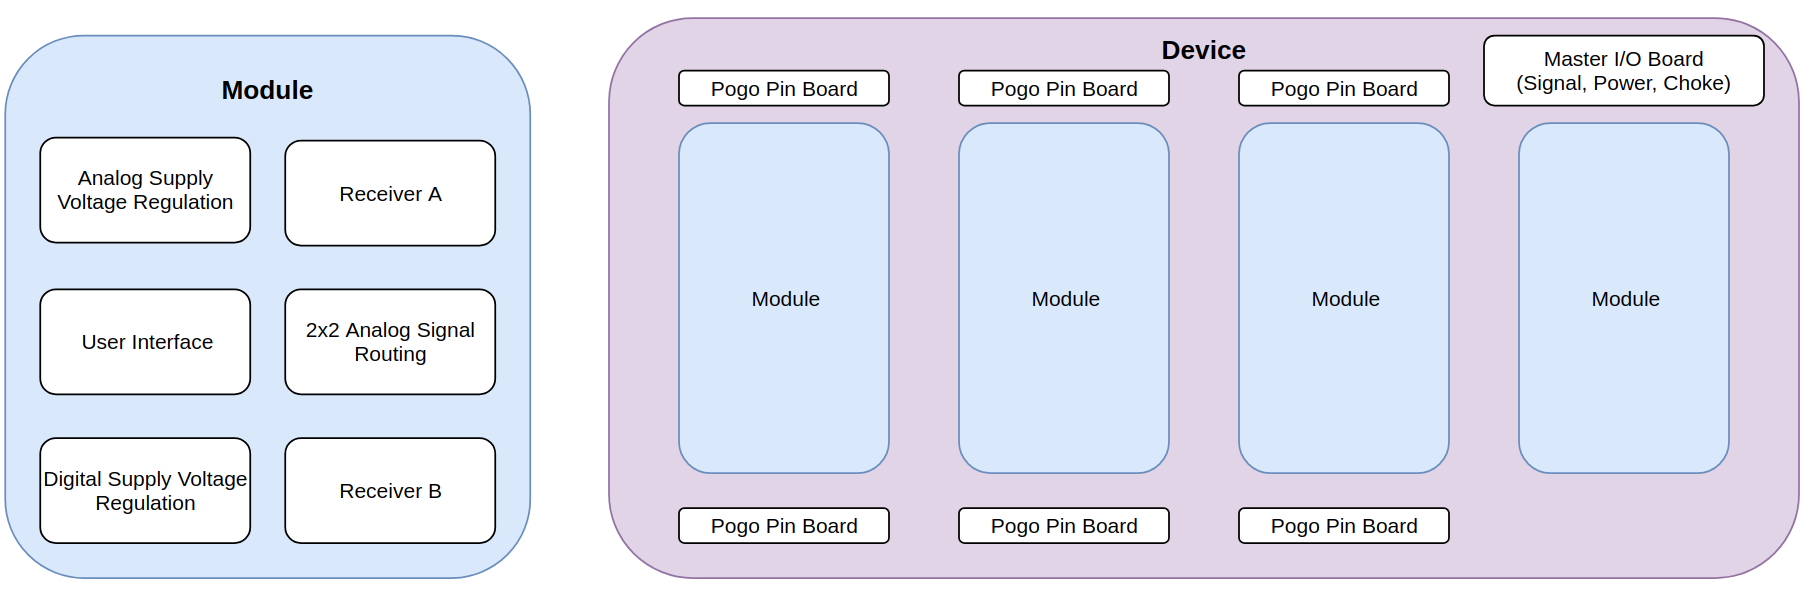
\includegraphics[width = \textwidth]{PR4Images/ModularHierarchy.png}
		\caption{Modular hierarchal design of the entire system.  On the right, the entire device is composed of four main modules and several other peripheral boards.  On the left, each module has several subsystems that are described in this document.  Note that the rightmost module in the full system does not use its receivers, so those components are depopulated.}
		\label{fig:systemhierarchy}
	\end{figure}

	This method would also allow a larger system to be constructed simply by connecting more of these modular boards (and increasing the maximum supply current of the power supply).  The following sections will detail the changes made to the prototype designs to accommodate this, as well as the new designs for the analog signal routing and user interface.

	\subsection{Microcontroller Selection}

	Though the prototype was initially designed for easy integration of the additional routing and user interface subsystems, the ATTiny40 is not adequate to support these.  The main issue with the ATTiny40 is its limited GPIO count.  In addition to the 16 pins required for the two receivers, fourteen pins must be allocated for the user interface and eight for the routing on each module.  This totals to 38, the minimum requirement for GPIO pins.  Extra pins for serial communications, debugging, and future potential connections should be included as well. 

	Another issue with the ATTiny40 was its lack of on-chip debugging capability.  Because of the device's focus on a limited feature set, it's proprietary TPI (Tiny Programming Interface) for programming did not support on-chip debugging via JTAG or similar \cite{ATTINY40datasheet}.  However, the programming interface should be compatible with Atmel's ICE in-system programmer which had already been purchased for use with the ATTiny40.  Other desirable features include an on-board oscillator to drive the clock for applications such as this that do not require a highly accurate clock, and 5V compatibility to interface easily with the existing system, most notably the relays.  This will reduce the number of external components necessary, minimizing cost and complexity.

	With these requirements, the ATMEGA3209-AFR was selected as the best option.  At \$1.47 a piece \cite{digikey}, the device is not quite as cheap as the PIC16F15385 (\$1.25 a piece), but it uses the same development tool chain as the ATTiny40 from before, which will make the switch of devices easier.  In a hand-solderable 48-TQFP package, this chip comes with 41 GPIO each capable of generating an interrupt, an internal 20 MHz oscillator, and a one-wire Unified Program Debug Interface (UPDI) which, as the name suggests, allows for in-system programming and debugging \cite{ATMEGA3209_datasheet}.

	\subsection{Receiver Subsystems}

	Adapting the receiver from the prototype into the module is fairly straightforward as a result of the prototype's success.  Each of the two receivers on board a single module has the same LM317 programmable voltage regulator set up as before.  The two receivers will share one LV8548MC dual H-bridge driver, which is driven by the ATMEGA3209.

	One major difference in the implementation is the mechanical configuration of the pogo-pins.  Because the pogo-pins were directly connected to the board on the prototype, much of the board area was wasted, with a major fraction of the surface devoted to the mechanical alignment of these electrodes.  This issue is even more important when designing the two-receiver module, as now the pins must be aligned for each of the receivers, meaning that the separation between the pins and hence the length of the circuit board must be no shorter than the height of one receiver.  To be more space efficient, the module will consist of a main board with all of the devices along with several remote boards connected via board-to-board connectors for the pogo-pins and user interface.  This will allow the mechanical placement of the main board to be independent (relatively) of the pogo-pins.  This will also reduce the vibrations and shocks to the main board as a result of the pogo-pins being depressed and released.

	\subsection{Analog Signal Routing}

	Each module will contain a two input, two output mixer.  Each of the two outputs 1 and 2 can be connected to either input $A$ or $B$, as well as the sum of the two inputs $A + B$.  Table \ref{tab:routing_outputs} shows the possible outputs.  As can be seen, there are only signals that must be available for the output.

	\begin{table}
	\begin{center}
	\begin{tabular}{ |c|c c| }
	\hline
	 Permutation & Output 1 & Output 2 \\ 
	 \hline
	 1 	& $A$ 	& $A$ \\  
	 2 	& $A$ 	& $B$ \\
	 3	& $A$ 	& $A+B$ \\
	 4	& $B$ 	& $A$ \\
	 5	& $B$ 	& $B$ \\
	 6	& $B$ 	& $A+B$ \\
	 7	& $A+B$ & $A$ \\
	 8	& $A+B$ & $B$ \\
	 9	& $A+B$ & $A+B$ \\
	 \hline
	\end{tabular}
	\caption{List of the $2^3$ possible output signals for each routing module.}
	\label{tab:routing_outputs}
	\end{center}
	\end{table}

	With this in mind, the specific implementation of the routing mechanism can be designed.  For the same reasons that relays were chosen to actuate the signal switching in the receiver subsystem, they should also be used here.  This is essential especially when an output is connected directly to an input, such as permutation 2 in Table \ref{tab:routing_outputs}, which will preserve both the SNR and frequency content of the signals in addition to the signal's output impedance.  However, when a summed output is chosen ($A+B$), the signals must necessarily pass through a summing amplifier, which will result in a low impedance output.  In this instance, the use of a mechanical relay is not strictly necessary.

	The specific implementation of the routing subsystem is shown in Figure \ref{fig:routingschem}.  Each output selector is in essence a three-to-one multiplexer.  The requirement for mechanical relays when the sum output is not selected requires the use of mechanical relays throughout, as each can only switch between two inputs.  Thus, each three-to-one multiplexer includes two of the same DPDT relays used for the receivers despite not all of the throws being in use, as they were cheaper than any SPDT relay.  Using the same EA2-5SNJ relays also minimizes additional components on the BOM.  The use of latching relays here is even more beneficial than in the receiver, as these relays will likely be set in a position for long periods of time, so the reduced current and heat dissipation compared to a non-latching relay is very beneficial.

	To generate the summed $A+B$ signal, a standard inverted summing amplifier is used.  The resistors were chosen to each be $10K\Omega$ so that each input is at unity gain.  Higher resistor values were avoided to reduce thermal noise.  However, the input impedance to the inverted amplifier is just the value of the input resistance, so non-inverting op-amp buffers are required to prevent preceding circuits on $A$ and $B$ from interacting with the summing amplifier.  As this already requires three op-amps and the output signal would be inverted, an additional unity gain inverted buffer is used at the output to re-invert the signal, resulting in $A+B$.

	This summing amplifier and related circuitry requires its own analog supply voltage.  In the worst case, the maximum voltage swing of each input signal $A$ and $B$ should be no more than 18Vpp, which is the maximum supply voltage available to a pedal from a receiver.  This means that the summing amplifier should ideally be able to swing 36Vpp.  However, the power supply currently being used provides 24VDC.  This means that without modification, the summing amplifier will not be able to sum all possible signals without clipping.

	There are several possible solutions to this issue.  One would be to change the device's power supply.  Moving to a chassis mount 48V supply like Mean Well's LRS-150-48 \cite{datasheet:LRS-150-48} (\$22.50 from Digikey \cite{digikey}) would allow for plenty of headroom and could provide much more current (in this case 3.3A), enough for six pedals each drawing 500 mA while leaving some budget for the device's own circuits.  A new power supply could be chosen to avoid the issue of switching noise in the audio range; the switching frequency of the LRS-150-48 is 65kHz, well above the audio spectrum.  Linear regulators could be used to drop the input voltage to the desired level, in this case just above 36V.  This supply could then be split with a resistive divider to provide the virtual ground needed for the op amp summer.  However, a chassis mount supply would involve introducing 120VAC wall voltages into the unit, which would not satisfy the SELV compliance specification.  Brick-type supplies in this voltage and current range are prohibitively expensive, such as the PSA120U-480L6 from Philhong USA for \$38 \cite{digikey}.

	A second option would be designing an on-board boost-buck converter to create the desired supply voltages.  In this case, this switching supply could be used to generate an arbitrary voltage, so a bipolar 18V or 24V set of rails could be created.  This would allow for sufficient headroom for the summing amplifier, and by virtue of the bipolar supply would not require AC coupling the summed signals to a virtual ground: they could remain DC coupled.  A switching supply would also be more efficient than a linear regulator.  However, the added complexity of implementing a switching voltage regulator, is probably not worth the benefits.  Noise from the on-board supply would need to be carefully controlled so as to avoid corrupting the audio signals.  In addition, a linear regulator would likely still be used to really clean up the residual ripple from a switching regulator.

	The third option is simply using a linear regulator to even out the current 24V supply and allowing the summing amplifier to clip at a lower voltage.  This is not as big an issue as it seems at first.  Though the worst case scenario is two 18Vpp signals being summed in phase, this would require the user to be using two pedals in 18V mode at full output level.  The more likely use case with two 9V pedals would work fine with the 24V supply.  If the user does cause the summing amplifier to clip, they can simply reduce the output level of the two pedals.  In addition, if the amplifier were able to sum two outputs to 36Vpp, this would cause the next pedal in the chain to clip as well because of its voltage could be 18V at maximum, so the 36Vpp output would only be usable at the input of the amplifier where it would not clip the amplifier input.  This is also the simplest option, as it requires only a linear regulator to clean up the 24V input and a resistive divider to generate the virtual ground reference voltage.  

	\begin{table}
	\begin{center}
	\begin{tabular}{|c|p{2.25in} p{2.25in}|}
	\hline
	Option & Pros & Cons \\
	\hline
	Change Power Supply 	& Allow increased headroom for summing amplifier.  Increase current capacity for entire system.  Possible to fix switching noise issue. 
								& Potentially expensive for quality supply with the required high current and voltage.  No guarantee that all issues will be solved. \\
	On-board Switcher 		& Bipolar supply possible for DC coupling.  Arbitrary headroom for this application.  More efficient than linear regulators. 	
								& Complicated.  Potential for its own noise issues would require mitigation. \\
	No Action 				& Easy.  Cheap.  Still satisfies most operating conditions. Low Noise.
								& Limited headroom.  Inefficient. \\
	\hline
	\end{tabular}
	\caption{Summary of analog supply voltage regulation options.}
	\label{tab:pwrsupplyproscons}
	\end{center}
	\end{table}

	Because of the simplicity of the third option and its relatively limited negative effects, this method was chosen to provide the supply for the summing amplifier.  To maximize the dynamic range of the summing amplifier, the regulated supply rail should be as close as possible to the 24V input.  The 200mV noise spec on the power supply means that the regulator must drop at least 200mV.  An adjustable regulator would be useful here to precisely set the output voltage.  The LM317 adjustable regulator used for the receiver is one option.  However, it's minimum 3V drop between input and output means that the analog supply rail cannot be set any higher than 21V \cite{LM317datasheet}.  This decreased headroom is not desirable, so a lower dropout device would be preferable.  The LM2931C is an adjustable low dropout voltage regulator which can be set output anywhere from 3 to 24V with a maximum dropout voltage of just 0.6V, about one diode drop.  This means that the analog supply voltage AVDD can be set very close to the 24V input.

	The LM2931C's datasheet provides design guidelines for setting the output voltage, but it follows the same principle as the LM317 divider used for the receiver.  The datasheet gives the following equation to set the output \cite{LM2931datasheet}:

	$$ V_{out} = V_{ref} \left( 1 + \frac{R_2}{R_1} \right) + I_{adj}R_2 $$

	which also accounts for the small current on the ADJ pin.  The datasheet also suggests keeping

	$$ 22.5k \ge \frac{R_1R2}{R_1 + R_2} $$

	According to the electrical characteristics page, the reference voltage $V_{ref} = 1.2V$, and the adjust pin current $I_{adj} = 0.2\mu$A.  Setting $R_1 = 27$k and $R_2 = 487$k gives an output voltage of 23V, which is ideal.  The 487k resistor is not one of the standard values, but slight adjustments in resistance to get to a nearby value cause too much of a change in voltage.  The output must also have a capacitive load on the order of 10$\mu$F for stability.  Figure \ref{fig:AVDDreg} shows the circuit implementation of the regulator.

	\begin{figure}
		\centering
		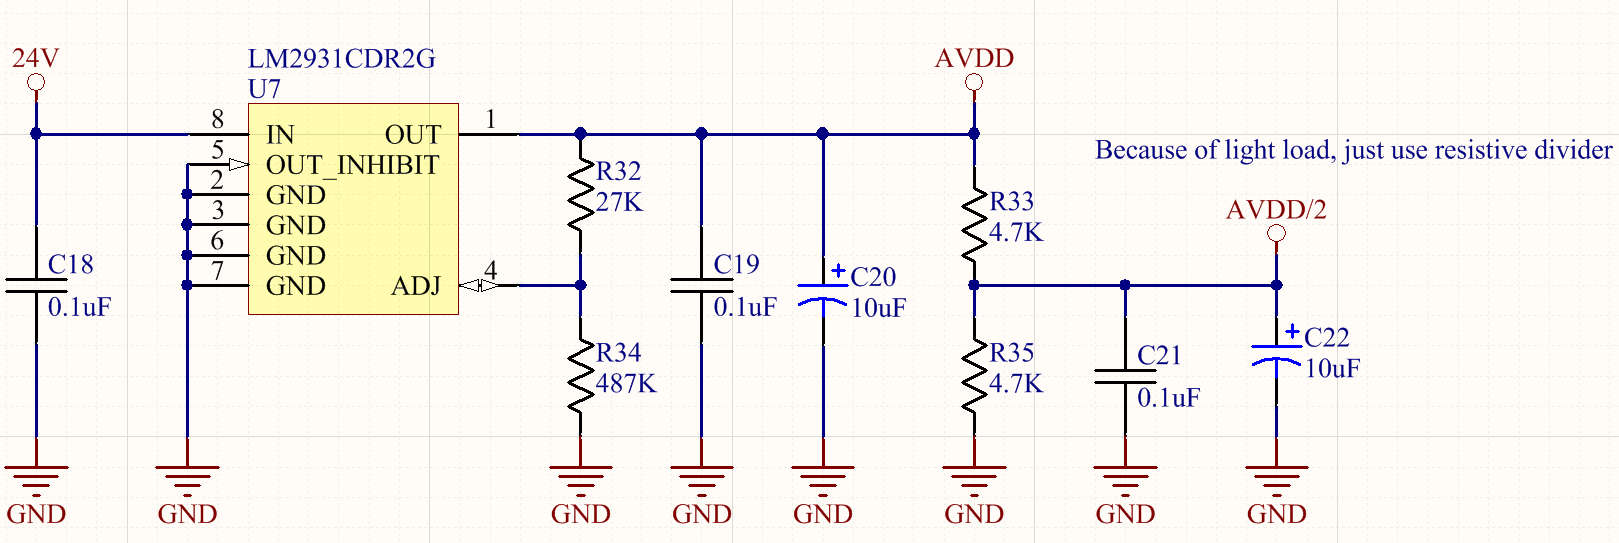
\includegraphics[width = \textwidth]{PR4Images/AVDDregulator.PNG}
		\caption{AVDD regulator design using LM2931C low voltage adjustable regulator and a resistive divider to provide a large split supply.}
		\label{fig:AVDDreg}
	\end{figure}

	From this analog supply voltage, a virtual ground can be produced from a simple resistive divider circuit.  Though in theory this is susceptible to sagging due to large current loads, this should not be an issue for this application because the reference voltage is connected only to the inputs of two op-amps, and tied to the audio signal through large resistors.

	The $A$ and $B$ inputs are each connected through a decoupling capacitor to their respective op-amp buffer inputs, and are pulled to the reference voltage via 1M resistors.  The 1M resistors were chosen to prevent the $A$ and $B$ signals from being heavily loaded down.  In the worst case, a signal could pass by eight of these buffer inputs, as show in Figure \ref{fig:worstcaserouting} without being buffered, so the equivalent resistance of eight of these pull-up resistors must not be too low.  The equivalent resistance of eight resistors in parallel is

	$$ R_{eq} = \frac{1}{\sum\limits_{i=1}^{8}\frac{1}{R}} = \frac{R}{8} $$

	\begin{figure}
		\centering
		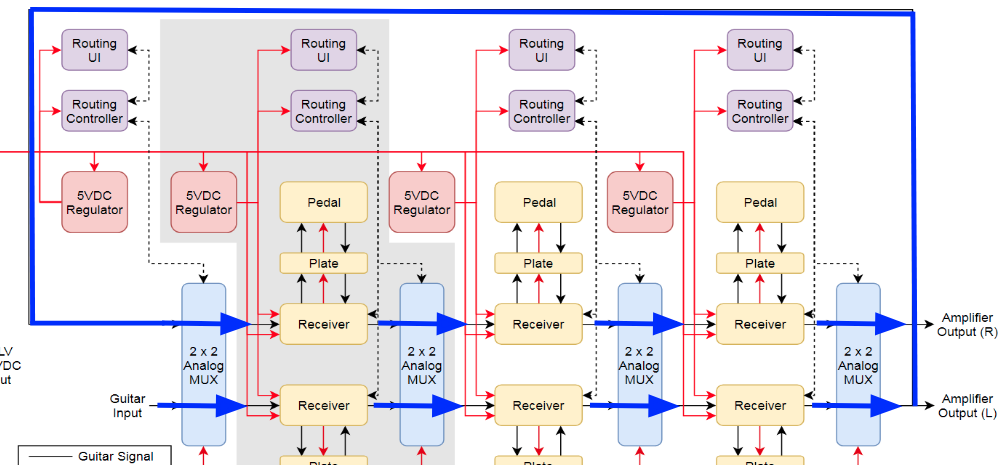
\includegraphics[width = 0.8\textwidth]{PR4Images/WorstCaseInputImpedancePath.png}
		\caption{The worst case routing path for input impedance sends the signal passed eight biasing resistors without ever being buffered.}
		\label{fig:worstcaserouting}
	\end{figure}

	so for 1M this is 125k$\Omega$.  Assuming a 10K$\Omega$ purely resistive output impedance from the guitar's pickups (on the high side for DC resistance but fairly reasonable for AC impedance), the input impedance is a bit too small for comfort.  Steps to mitigate this issue should be taken. A large resistor value here also means the capacitance of the decoupling capacitor can be less to maintain a similar cutoff frequency, and it will be cheaper to have a higher quality plastic film or C0G ceramic capacitor in a smaller value.  The limit to choosing a very large resistor is the thermal noise, which may become a concern even with this value.  If this becomes an issue, the values can be adjusted once the board has been fabricated.  The cutoff frequency for the high pass filter formed by pull-up resistor and the decoupling capacitor should have its cutoff frequency on the order of 5-10Hz so it will pass the full audio range.  For a 1M resistor, this means

	$$ C = \frac{1}{2\pi R F_c} = \frac{1}{2\pi (1 \text{M}\Omega) (10 \text{Hz})} = 15.8 \text{nF}$$

	Because this is on the high end of the frequency range, the next larger standard value capacitor, 0.022uF, is used.  Kemet offers a 0.022uF film capacitor in through hole mounting for just \$0.25.  The film capacitors are more linear and have lower ESR and self inductance than typical ceramic caps, making them suitable for audio signal path usage.  The resistors can be standard.

	The op-amp selected should have low noise, low input bias current to prevent loading the input signal lines, and a rail-to-rail output to maximize headroom.  For op-amps compatible with a supply of 24V or more, Texas Instrument's OPA1679IDR is a good candidate.  At \$1.20 from Digikey, it is not cheap, but its datasheet claims 0.0001\% THD+N, a 10 pA max input bias current, and voltage output within 800mV of each rail \cite{OPA1679IDRdatasheet}.  These specs compare admirably to the TLV4172IDR and OPA4172IDR, each of which are twice the price.  Because there are not too many components in the audio path and its value as a reliable reference is paramount, it is appropriate to use more expensive and higher quality parts here.  The schematic for the analog signal routing subsystem is shown in Figure \ref{fig:routingschem}.  

	\begin{figure}
		\centering
		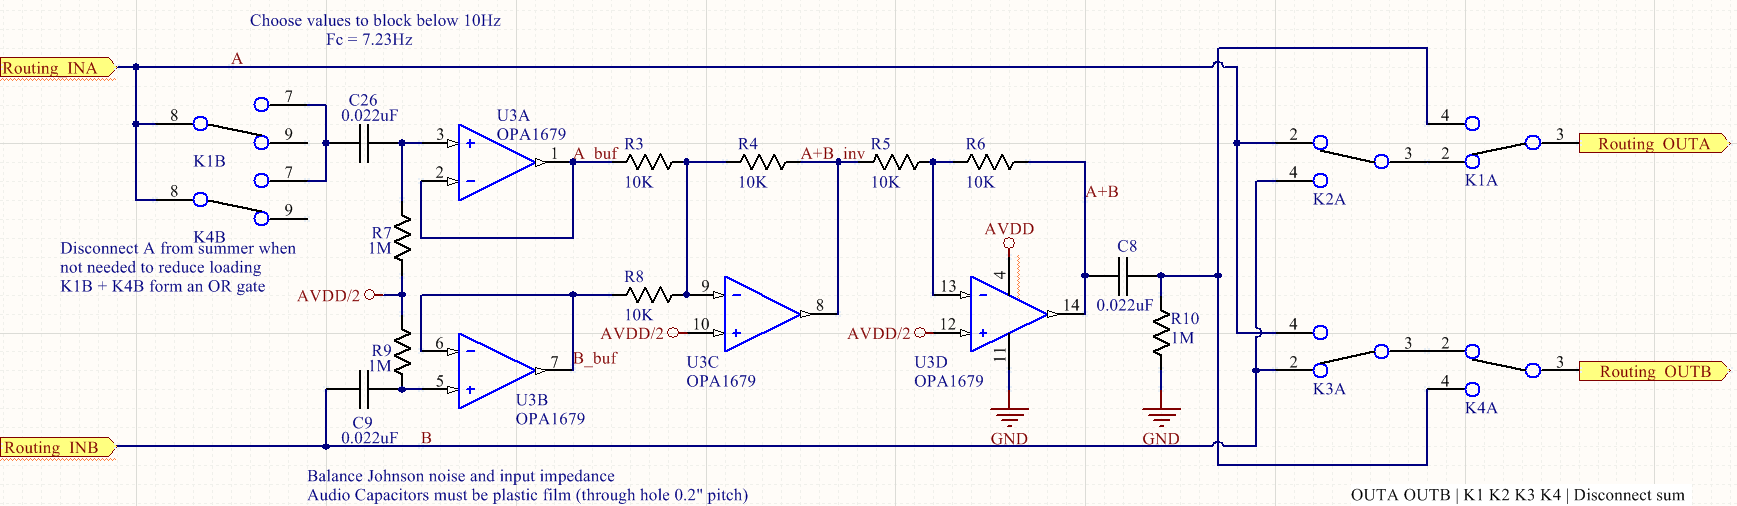
\includegraphics[width = \textwidth]{PR4Images/RoutingSchem.PNG}
		\caption{Schematic of analog signal routing subsystem.  Note that the second halves of two out of the four routing relays are in use.  The relays associated with choosing between a summed output or not are used to create an OR gate which will disconnect the biasing resistors from the $A$ signal, reducing the loading whenever the summer is not needed.}
		\label{fig:routingschem}
	\end{figure}

	\subsection{User Interface}

	The above analog signal routing subsystem needs to be controlled by the user.  Because this device is designed to simplify the user experience, the user interface should be intuitive to use; no or few instructions should be needed to operate it.  The user interface should clearly indicate the current state of the signal routing, and the method by which the user can change the routing should be likewise linked to the physical signal connections being made.  To avoid disrupting the user from their focus on audio, the interface should be primarily visual and tactile in nature, as opposed to auditory.  For these reasons, the indication and actuation elements should be meshed, taking the form of push buttons with an integrated light.

	As described in Table \ref{tab:routing_outputs} above, each of the two inputs can be connected to each of the two outputs.  This includes cases where both inputs are connected to one or both of the outputs.  In no scenario can an output be connected to no input, which means that the user will never experience any "dead spots" where no sound can be heard.

	Qualitative tests were used to determine the effectiveness of such an indicator light.  An 8" $\times$ 1/2" $\times$ 1/4" clear acrylic sheet was cut using a laser cutter.  One side of this sheet was engraved with the same laser cutter in a continuous pattern to provide a rough surface off which light can reflect and refract.  A white LED was lit and place on one end of the sheet, facing the 1/2" $\times$ 1/4" rectangular side.  When the LED was held within 5mm or so of the face, the acrylic appeared to illuminate when viewing either of the 8" $\times$ 1/2" faces.  This rapid prototyping was conducted in a brightly lit machine shop, with lighting conditions similar to that expected in a guitar retail store.

	\begin{figure}
		\centering
		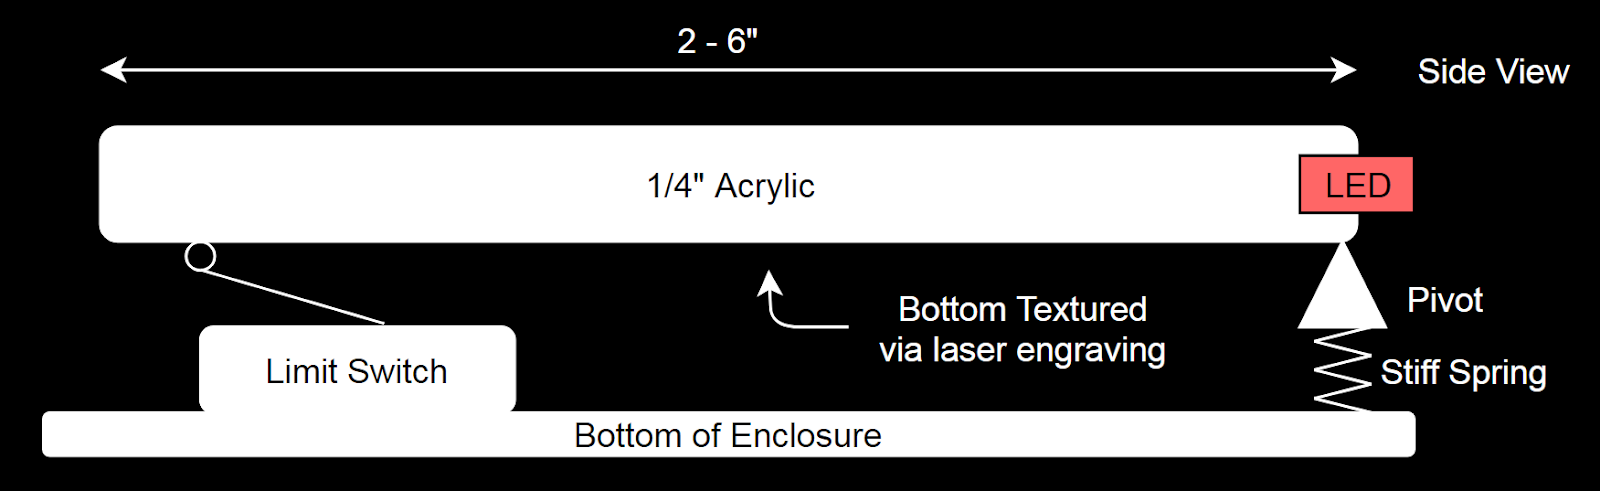
\includegraphics[width = 0.8\textwidth]{PR4Images/oldUIsideview.png}
		\caption{Side of view sketch of the user interface design.}
		\label{fig:UIsketch}
	\end{figure}

	Though specific mechanical design for this switch, as with the rest of the completed unit is not yet complete, the basic design is shown in Figure \ref{fig:UIsketch}.  As with the rapid prototype test described above, the central component of the subsystem is a beam made of clear 1/4" acrylic with the bottom side textured via laser cutter.  This beam functions as the light pipe used to direct and then scatter light from an LED, converting this light from a single source to an illuminated shape.  A white LED is inserted in a hole drilled on the smallest face of the beam, pointing down the length of the beam.  This hole should be centered on the face and is 3mm in diameter to fit a 3mm diameter LED.  The LED is connected via a twisted pair of wires to the main PCB (not shown), where it is powered by a constant current source.

	As mentioned, the acrylic beam's bottom is textured to allow the light from the LED to reflect and refract.  The acrylic rests on a longer aluminum beam for added support.  Between these is a thin layer of white vinyl or paper attached by pressure-sensitive adhesive to visually isolate the acrylic light from the underlying support structure.  Under one end of the acrylic, the aluminum beam sits on a limit switch actuator, which is used to detect when the user has depressed the acrylic beam.  On the opposite end, the aluminum extends beyond the extent of the acrylic.  The aluminum beam is pivoted on this end via a through hole.  This system is more clearly described in the force body diagram in Figure \ref{fig:UIFBD}.

	\subsubsection{User Interface Force-Body-Diagram and Switch Selection}

	\begin{figure}
		\centering
		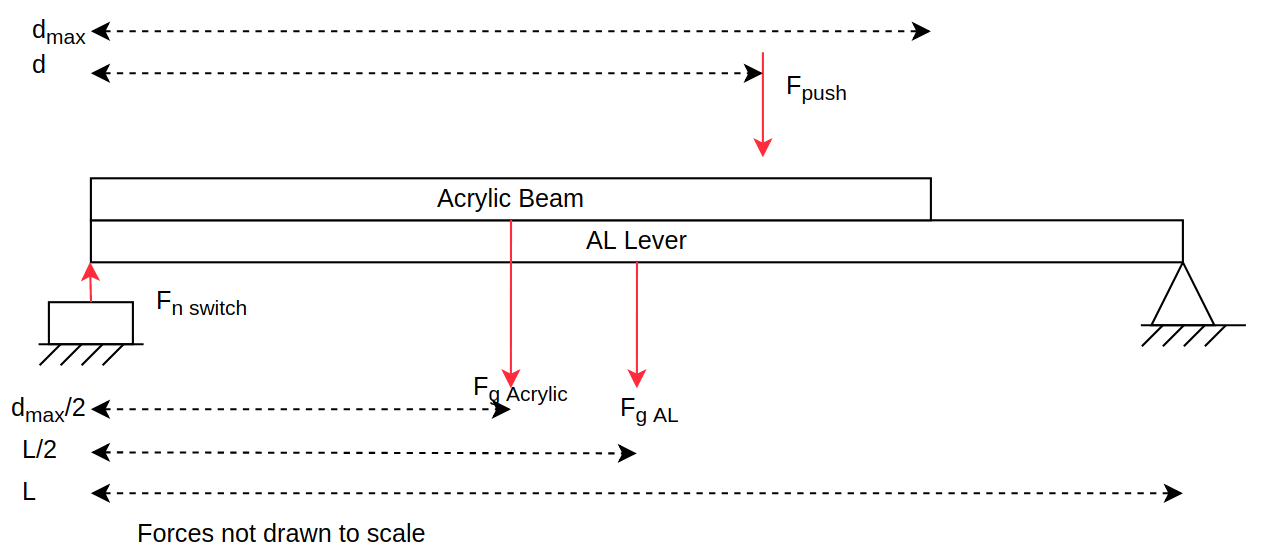
\includegraphics[width = 0.8\textwidth]{PR4Images/UIFBD.png}
		\caption{Force-Body Diagram demonstrating the torque relation between forces.}
		\label{fig:UIFBD}
	\end{figure}

	As can be seen, designing the system is simply a matter of balancing the torques on the beam.  Assuming no deflection of the beam, which is reasonable given the small magnitude of the forces and distances involved compared to the rigidity of the aluminum and even acrylic, and no friction, the system can be described in a static, undisturbed state by

	$$ F_{limit} l \ge F_{g_{AL}} \frac{l}{2} + F_{g_{acrylic}} \left( l - \frac{d_{max}}{2} \right) $$

	This requires that the torque produced by the operation force of the limit switch is greater than the torque produced by the weight of the beam.  Assuming an 8" $\times$ 1/2" $\times$ 1/4" piece of aluminum (this is on the larger side, which will give some margin for the limit switch force requirement), and the density of aluminum 2.7 g/cm$^3$ \cite{SolidsDensities}, 

	$$ F_{g_{AL}} = m_{AL}g = \left(16.39\text{cm}^3\right) \left(2.7 \text{g/cm}^3 \right) \left( 10^{-3}\text{kg}/\text{g} \right) \left( 9.8 \text{m/s}^2 \right) = 0.43 \text{N} $$

	A 6" $\times$ 1/2" $\times$ 1/4" (again also on the larger side) piece of acrylic with density 1.2 g/cm$^3$ \cite{SolidsDensities} would have weight

	$$ F_{g_{acrylic}} = m_{acrylic}g = \left( 12.29\text{cm}^3 \right) \left( 1.2 \text{g/cm}^3 \right) \left( 10^{-3}\text{kg}/\text{g} \right) \left( 9.8 \text{m/s}^2 \right) = 0.14\text{N}$$

	This means that the minimum required normal force by the limit switch before it activates is

	$$ F_\text{sw} \ge \frac{(l/2)0.43\text{N} + (l-d_\text{max}/2) 0.14\text{N}}{l} $$

	and is dependent on the specific geometry of the lever.  An upper bound can be found by substituting $l$ for all of the distances, which means that the operating force of the limit switch must be greater than the sum of the weights of the acrylic and aluminum, so $F_\text{sw} \ge 0.57\text{N}$, though something a little higher like 1N might be a good lower bound for the switch operating force to leave some margin.  On Digikey, switches' operating force is given in units of gram-force $gf$ where $1gf = 0.00980665\text{N}$ so this lower bound of 1N = $101gf$.

	The upper bound for the switch operating force is limited by the force required to depress the switch by the user when they press closest to the pivot, or at distance $d_\text{max}$ from the end of the lever furthest from the pivot.  Again this is dependent on the relative lengths and geometry of the design.  Keeping the acrylic beam as short as possible will reduce the difference in force required to activate the switch along its length.  As with the rest of this mechanical system, more work will be done once the PCB design has been sent out for manufacturing.  Because this design does not need to be completed before the PCB is designed and manufactured, this does not pose an issue with the timing of the project.

	\subsubsection{Button Layout}

	With these unified indicator-buttons, the remaining design for the user interface is the exact layout of the buttons.  As mentioned, they should be physically intuitive for the user to select the active inputs for each output.  The physically layout of the receivers is on a $3 \times 2$ grid.  The signal routing subsystems are used to connect the paired receivers on adjacent columns.  Figure \ref{fig:OverallUILayout} shows the overall layout of the receivers and the buttons.

	\begin{figure}
		\centering
		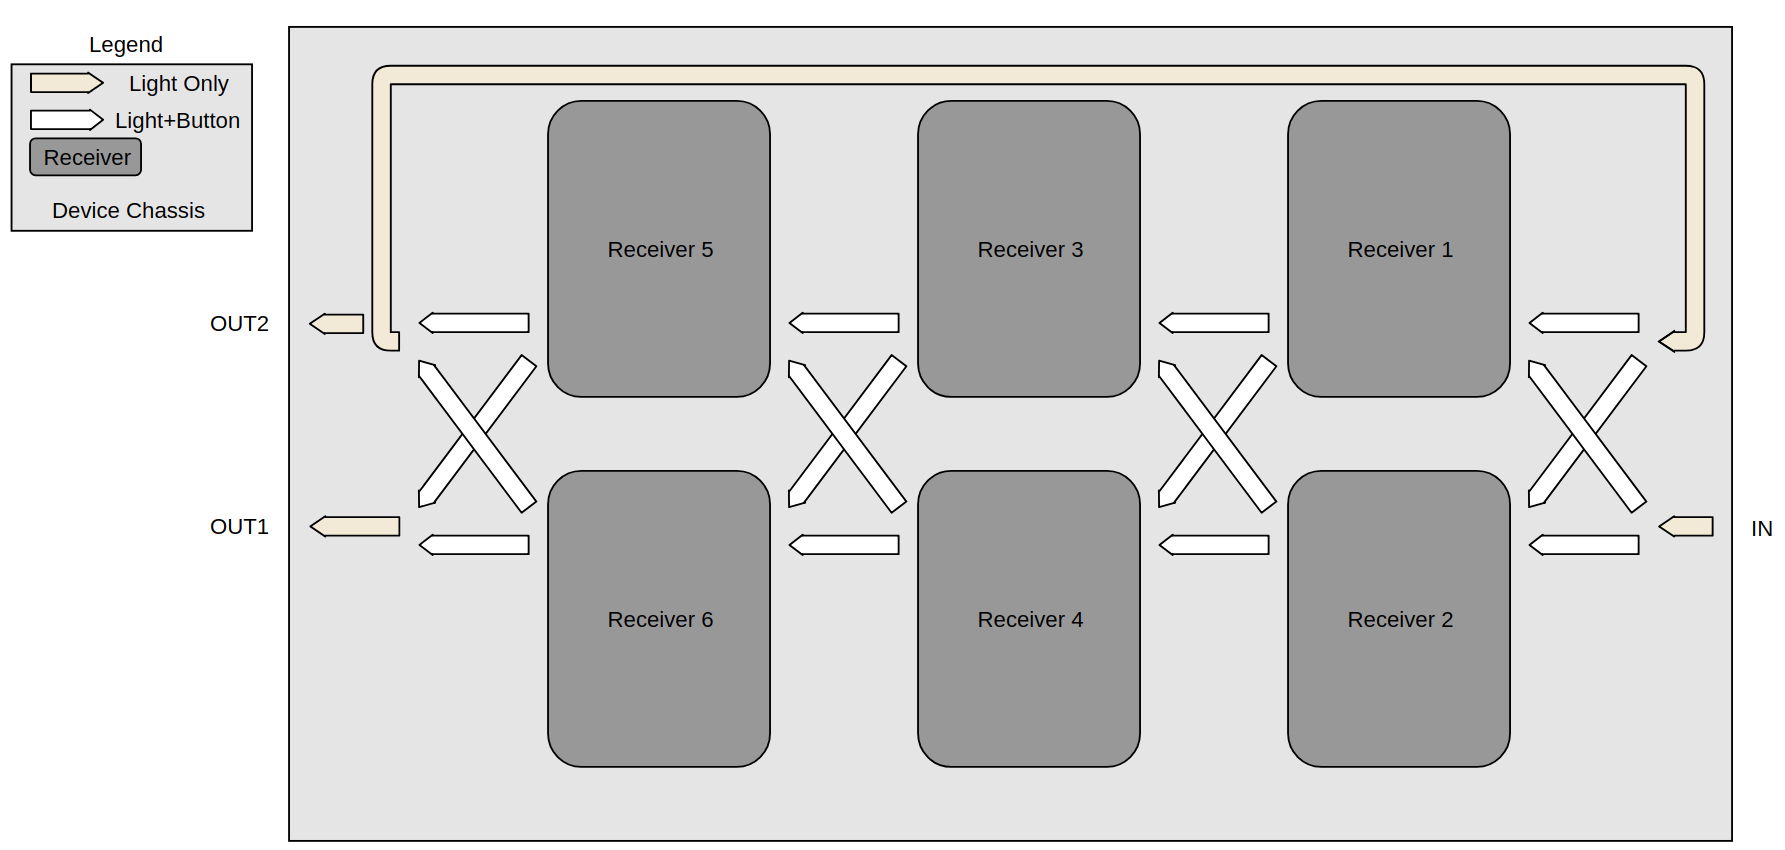
\includegraphics[width = \textwidth]{PR4Images/UIOverview.png}
		\caption{Overview of the user interface for understanding the physical layout of the overall unit.}
		\label{fig:OverallUILayout}
	\end{figure}

	To conform with guitar effects industry standards, the signal flow for the overall unit is from right to left.  Between each vertical pair of receivers (such as Receivers 1 and 2 in Figure \ref{fig:OverallUILayout} is a set of four integrated buttons and indicators, shown as white arrows.  Each set of these white arrows is connected to one module board and the board's routing subsystem.  Each button in the set is related to one particular signal routing direction.  For example, the arrow that points left from Receiver 2 to Receiver 4 indicates if the output of Receiver 2 is available on the input of Receiver 4.  In this example, that indicator would be lit if Receiver 4's input was either the output of Receiver 2 or the sum of the outputs of Receiver 1 and Receiver 2.  Each arrow shaped button toggles the state of both its LED and the relays associated with its connection.  In addition, there are a few lights, shown as tan arrows, that do not function as switches, and are lit depending on certain parameters.  For example, the indicators for IN, OUT1, and OUT2 are lit when a cable is plugged into the respective output to show that the connection has been correctly made.  In normal operation at a music store, the output will remain plugged in, so this will function as a de facto ON/OFF indicator.  The large indicator representing the feedback path will be turned on only when the feedback path is active: at least one of the two white arrows on the far right that point from the end of the feedback indicator into Receiver 1 and Receiver 2 are lit.

	\subsubsection{Control Finite State Machine}

	Each routing subsystem is a two input, two output mixer.  Each of the outputs can be the connected to either input or the sum of the inputs.  This means that these outputs can be controlled independently, so each set of white arrows can be split into two groups based on the output they control.  For instance, in Figure \ref{fig:UIarrowlabels}, buttons $a$ and $b$ control the top output while $c$ and $d$ control the bottom output.

	\begin{figure}
		\centering
		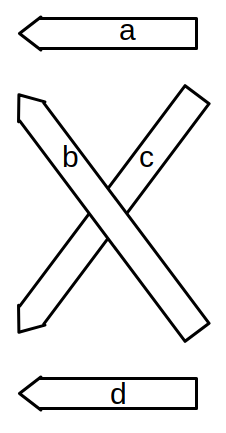
\includegraphics[width = 0.15\textwidth]{PR4Images/UIarrowlabels.png}
		\caption{Set of button-indicators.  These are associated with one module and are used to control the module's signal routing subsystem.  The letters are used for identification in this document.}
		\label{fig:UIarrowlabels}
	\end{figure}

	The switch logic and debouncing will be computed on the microcontroller.  The finite state machine depicted in Figure \ref{fig:UIFSM} will run in two instantiations on the microcontroller to cover the $a$ and $b$ set of switches along with the $c$ and $d$ set.  This diagram illustrates only the machine associated with the $a$ and $b$ switches.  This is Moore state machine where the output is determined by the current state.  The output/state is written in the boxes, and is described by STATE[1:0] where the bit 1 is the state of indicator $a$ and bit 0 is the state of indicator $b$.  The input vector is INPUT[1:0] where bits 1 and 0 represent whether switches $a$ and $b$ are asserted at any given time.

	\begin{figure}
		\centering
		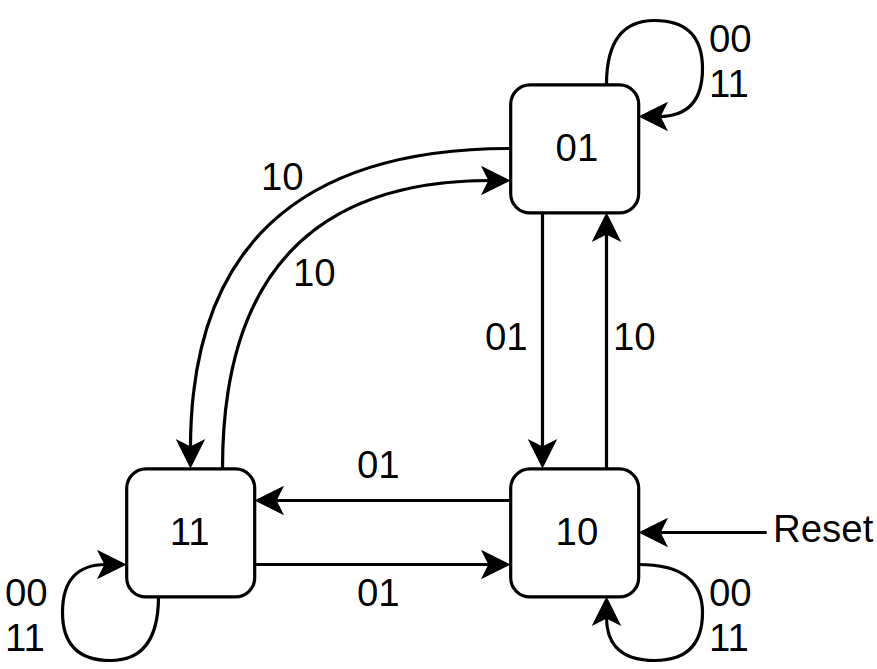
\includegraphics[width = 0.5\textwidth]{PR4Images/UIFSM.png}
		\caption{Finite State Machine describing the operation of the user interface for the signal routing.}
		\label{fig:UIFSM}
	\end{figure}

	As can be seen, the machine always starts in state $\mathtt{10}$, which means that the top input is connected to the top output in a "straight" line.  In terms of Figure \ref{fig:OverallUILayout}, this means that the unit will route the signal

	$$ \text{RECEIVER 1} \rightarrow \text{RECEIVER 3} \rightarrow \text{RECEIVER 5} $$

	This diagram does not indicate any information about the state of the relays in the actual signal routing subsystem.  This is because each FSM state, which is nominally tied to the LED state, also has a dedicated setting for those relays.  All of this information is summarized in a state transition table shown in Table \ref{tab:FSMtransitions}.  Note that state $\mathtt{00}$ should never be reached, as this would indicate that no output is currently selected.  If this state does mistakenly appear, it should transition to state $\mathtt{10}$, which is the default starting state.

	\begin{table}
	\begin{center}
	\begin{tabular}{ |c c|c c|c c|c c|}
	\hline
	\multicolumn{2}{|c|}{State/LED State} & \multicolumn{2}{|c|}{Relay Position} & \multicolumn{2}{|c|}{Input} & \multicolumn{2}{|c|}{Next State} \\
	\hline
	$a(d)$ & $b(c)$ & K1(K4) & K2(K3) & $a(d)$ & $b(c)$ & $a(d)$ & $b(c)$ \\
	\hline
	0 & 0 & 0 & 0 & X & X & 0 & 1 \\
	\hline
	\multirow{3}*{0} 	& \multirow{3}*{1} 	& \multirow{3}*{0} 	& \multirow{3}*{1} 	& 0 & 0 & 1 & 0 \\
						& 					&					&					& 0 & 1 & 1 & 0 \\
						& 					&					&					& 1 & 0 & 1 & 1 \\
						& 					&					&					& 1 & 1 & 0 & 1 \\
	\hline
	\multirow{3}*{1} 	& \multirow{3}*{0} 	& \multirow{3}*{0} 	& \multirow{3}*{0} 	& 0 & 0 & 1 & 0 \\
						& 					&					&					& 0 & 1 & 1 & 1 \\
						& 					&					&					& 1 & 0 & 0 & 1 \\
						& 					&					&					& 1 & 1 & 1 & 0 \\
	\hline
	\multirow{3}*{1} 	& \multirow{3}*{1} 	& \multirow{3}*{1} 	& \multirow{3}*{X} 	& 0 & 0 & 1 & 1 \\
						& 					&					&					& 0 & 1 & 1 & 0 \\
						& 					&					&					& 1 & 0 & 0 & 1 \\
						& 					&					&					& 1 & 1 & 1 & 1 \\
	\hline
	\end{tabular}
	\caption{Routing User Interface FSM transition table.  The table describes the states for the $a$ and $b$ switches, and with the $c$ and $d$ side in parenthesis.}
	\label{tab:FSMtransitions}
	\end{center}
	\end{table}

	The embedded software running on the ATMEGA3209 will consist of two of these state machines, as well as two of the state machines that define the receiver operation.

	\subsubsection{Electrical Design}
	The electrical hardware design of the user interface is very simple.  The buttons are connected directly between pins on the ATMEGA3209 and ground, and pull down the inputs when they are activated.  The more interesting facet are the LED drivers.  They use a standard constant current LED driver circuit, controlled from the microcontroller.  Because the ATMEGA3209 has a limited maximum ground current, it cannot be used to drive the LEDs directly.  White LEDs are used for visual effect, and they are typically specified for a forward current of 20mA.  Figure \ref{fig:LEDdriver} shows the circuit.  The LED has a 3V forward voltage drop and should have a 20mA forward current.  This means that the collector voltage of the BJT may be no greater than 2V given the 5V supply.  Choosing an emitter voltage of 1.5V allows for a 500mV drop from the collector to the emitter to allow for variations in LED forward voltage.  R24 is used to set the current given this emitter voltage.  Because the base voltage should be one diode drop above the emitter, the resistive divider formed by R40 and R42 set the base voltage to be 1.9V.  A $\beta$ of 100 suggests that the base current will be 200$\mu$A.  This constant current source should keep the LEDs lit evenly.

	\begin{figure}
		\centering
		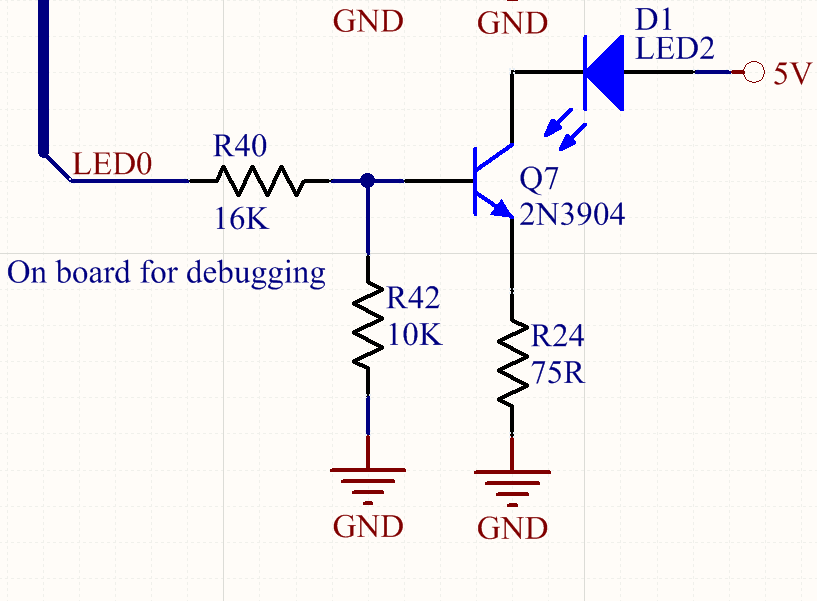
\includegraphics[width = 0.5\textwidth]{PR4Images/LEDconstcurrentdriver.PNG}
		\caption{Constant current source for LED.}
		\label{fig:LEDdriver}
	\end{figure}


\section{Logistics}

	\subsection{Updated Schedule}

	Note: \colorbox{green}{Green text} indicates complete work.  \colorbox{yellow}{Yellow text} indicates work in progress.  \colorbox{red}{Red text} indicates items that are behind schedule.

	The schedule up to weeks 19 and 20 has been colored in to reflect changes since Progress Report 2.  From the current date forward, the schedule is given weekly with realistic timeline goals

	\begin{table}[H]
	\begin{tabular}{llp{4in}}
	Weeks    & Dates         & Plan \\
	\hline
	1 \& 2   & 9/2 - 9/15    &  \colorbox{green}{Complete and revise Project Proposal and meet with advisers}      \\
	3 \& 4   & 9/16 - 9/29   &  \colorbox{green}{Conduct experiments described above to help refine specifications.}  \color{green}Begin higher level block diagrams of system.  Progress Report \#1 due 9/28     \\
	5 \& 6   & 9/30 - 10/13  &  \color{green}Begin prototyping key features, such as pedalboard - plate interface. Rapid prototyping of features such as plate design to inform first prototype. Develop lower level block diagrams and begin schematic design.     \\
	7 \& 8   & 10/14 - 10/27 &  \color{green}Electronic and Mechanical CAD design for first prototype.  The first prototype will be a single slot for testing the 1) reliability of electrical connections between plate and board, 2) mechanisms for attaching pedal to plate (mechanical and electrical), 3) strength of magnets needed to hold plate to board, 4) method for hot-swappable bypassing (sensing and actuation)     \\
	9 \& 10  & 10/28 - 11/10 & \color{green}Complete ECAD and MCAD design of single receiver prototype.  Progress Report \#2 due 11/5    \\
	11 \& 12 & 11/11 - 11/24 &  \color{green}Begin fabrication of PCB, mechanicals.  Write code for receiver microcontroller.  In parallel, begin schematic design for full scale Prototype 2.  \\
	13 \& 14 & 11/25 - 12/8  & \color{green}Fabricate mechanical parts.  Assemble circuit boards.  Perform preliminary testing on first prototype.      \\
	15 \& 16 & 12/9 - 12/22  &  \color{green}Continue testing and analyze results.  Outline goals/changes for next iteration.  Oral Design Review/Presentation 12/10    \\
	17 \& 18 & 12/23 - 1/5   &  \color{green}Winter Break: Expect Little Progress    \\
	\end{tabular}
	\end{table}

	\begin{table}[H]
	\begin{tabular}{llp{4in}}
	Weeks to Go   & Start Date         & Plan \\
	\hline

	7 & 2/15 &  Complete PCB layout by 2/18.  Send PCB for fabrication on 2/19.  Rapid prototype UI switches.  Design major MCAD components.  Schedule swap time experiments for next week.\\
	6 & 2/22 &  Design peripheral boards (pogo pins, master I/O).  Fabricate peripheral boards with milling machine.  Finish MCAD by 2/25. Begin software for routing and UI. \\
	5 & 3/1  &  Receive boards from fabrication.  Populate, debug them.  Full software integration and testing.  \\
	4 & 3/8  &  Fabricate enclosure.  Assemble entire device.  Perform functional and signal quality tests.  Progress Report \#5 due 3/8.  \\
	3 & 3/15 &  Perform remaining tests.  Analyze data. If necessary make modifications to PCB design and send for fabrication immediately.   \\
	2 & 3/22 &  Make last minute adjustments.  Prepare for presentation.  Write final report.  Final Oral Presentation 3/25  \\
	1 & 3/29 &  Revise final report.  Final Written Report due 4/5.    
	\end{tabular}
	\end{table}

	The schedule is tight but should the project should be accomplished in time for a live demonstration at the final presentation.

	\section{Updated Budget}

	The cost of the system has not been a major issue so far.  Pending completion of the bill of materials for the full system design, the additional required per module electronics components should not total more than \$50.  The phono plugs needed for the plates should cost another \$40.  The PCB manufacturing for five 4"x6" boards should be about \$60 if they remain 2 layer (double that for 4 layers).  Mechanical design parts are minimal, as scrap material is used as much as possible.  Thus, for four modules, the cost will be 

	$$ (4)\$50 + \$40 + \$60 = \$300 $$

	With less than \$100 spent on the first prototype, this leaves room for an emergency last minute board spinning and other small incidentals.

\newpage
\bibliographystyle{plain}
\bibliography{ThesisSources}

\section{Appendix}
Attached is the entire schematic design for the full scale design.  Because it is constantly being updated, some of the details may not exactly match those discussed in this document.  This schematic is the current state of the project.


\end{document}
